\documentclass[12pt, a4j]{ltjsarticle}
\usepackage{luatexja-fontspec}
\usepackage{amstext, amsmath, amssymb, amsthm}
\usepackage[morisawa-pr6n, bold]{luatexja-preset}
\usepackage[scaled = 1.03]{helvet}
\usepackage[top = 2cm, bottom = 2cm, left = 2cm, right = 2cm]{geometry}
\usepackage{mathtools}
\usepackage[dvipdfmx]{graphicx}
\usepackage{fontspec}
\usepackage{mathrsfs}
\pagestyle{empty}
\renewcommand{\baselinestretch}{1.6}
\newtheorem{thm}{定理}
\newtheorem{lem}[thm]{補題}
\newtheorem{defi}[thm]{定義}
\newtheorem{axm}[thm]{公理}
\newtheorem{cor}[thm]{系}
\newtheorem{alg}[thm]{アルゴリズム}
\newtheorem{exm}[thm]{例題}
\allowdisplaybreaks

\usepackage{listings, color}
%\usepackage{jlisting}
\definecolor{OliveGreen}{rgb}{0.0,0.6,0.0}
\definecolor{Orange}{rgb}{0.89,0.55,0}
\definecolor{SkyBlue}{rgb}{0.28, 0.28, 0.95}
\definecolor{AtomDark}{rgb}{0.15, 0.17, 0.2}
\lstset{
  language={Python}, % 言語の指定
  basicstyle={\ttfamily},
  identifierstyle={\small},
  commentstyle={\smallitshape},
  keywordstyle={\small\bfseries},
  ndkeywordstyle={\small},
  stringstyle={\small\ttfamily},
  frame={tb},
  framesep=2\zw,
  breaklines=true,
  columns=[l]{fullflexible},
  numbers=left,
  xrightmargin=0\zw,
  xleftmargin=3\zw,
  numberstyle={\scriptsize},
  stepnumber=1,
  numbersep=1\zw,
  lineskip=-0.5ex,
  keywordstyle={\color{SkyBlue}},     %キーワード(int, ifなど)の書体指定
  commentstyle={\color{OliveGreen}},  %注釈の書体
  stringstyle=\color{Orange}        %文字列
}
\newcommand*{\cd}{{\rm cd}}
\newcommand*{\lcm}{{\rm lcm}}
\newcommand*{\NN}{\mathbb{N}}
\newcommand*{\ZZ}{\mathbb{Z}}
\newcommand*{\SS}{\vspace{1cm}}
\newcommand{\bm}[1]{{\mbox{\boldmath $#1$}}}


\begin{document}
%\input{head}
\tableofcontents
\newpage
\section{序論}
\subsection{概要}
AtCoderなどで競技プログラミングをしているので、課題ついでに競プロ用のライブラリを整備します。競技プログラミングでは速度が問われ、一からアルゴリズムを実装していると間に合わないことがあります。一方で、ライブラリを貼るだけで通る問題はほとんどなく、それを理解して応用できる力がある必要があり、コードを理解しつつコンテスト中に競プロの本質的な部分に集中できるようライブラリを整備していこうと思います。

\subsection{環境}
実際にAtCoderでサポートされている言語バージョンに準じて作っていきます。PythonとPyPyがサポートされています。
\\
\begin{lstlisting}
# On AtCoder's Custom Code Test
import sys
print(sys.version)

import pkg_resources
for e, dist in enumerate(pkg_resources.working_set):
    print(dist.project_name, dist.version, end = ", " + "\n" * (e%8 == 7))

>> Python
3.8.2 (default, Feb 26 2020, 02:56:10)
[GCC 7.4.0]
..., scipy 1.4.1, ..., numpy 1.18.2, numba 0.48.0, networkx 2.4, ...

>> PyPy
3.6.9 (7.3.0+dfsg-1~ppa1~ubuntu18.04, Dec 24 2019, 08:12:19)
[PyPy 7.3.0 with GCC 7.4.0] ...
\end{lstlisting}

簡単に言えば、Python は ver.3.8, PyPy は Python ver.3.6 のものが埋め込まれており、PyPy は定数倍高速化が超強力な代わりに numpy, scipy, numba, networkx などのサードパーティーライブラリは使用できない。
\\
\begin{lstlisting}
!apt-get install pypy
!apt install texlive-fonts-recommended texlive-fonts-extra cm-super dvipng
\end{lstlisting}
\quad\\
で Google Colab に PyPy, $\LaTeXe をインストール。$

\subsection{その他}
基本的に Google Colab のコードと同じものを載せていますが、都合上一部省略あるいは増強したものがあります。
またより厳密で詳細な証明を書いていることもあります。

\newpage
\section{基礎的で非アルゴリズム的なもの}
\subsection{入力高速化}
\\
\begin{lstlisting}
import sys
input = sys.stdin.readline
\end{lstlisting}
\quad\\
入力が $10^5$ 行を超える場合、 \lstinline{sys.stdin.readline} に置換することで大きく高速化できる。
ただし \lstinline{open(0)} の方が高速化されることも多い。
\quad\\

\subsection{再帰制限の変更}
\\
\begin{lstlisting}
import sys
sys.setrecursionlimit(50000)
\end{lstlisting}
\quad\\
Pythonでは再帰上限が $1000$ 回に設定されており、これを超えると \lstinline{RecursionError: maximum recursion depth exceeded in comparison} を出す。
\lstinline{sys.setrecursionlimit(n)} で上限を $n$ 回に設定しこれを回避できる(ただし、メモリに負荷がかかり、ある程度超えるとPythonがクラッシュすることには変わりないので、乱用に注意)。
\newpage

\subsection{タイマーのセット}
\\
\begin{lstlisting}
def timer(func, v, *args, **kwargs):
    import time
    if __name__ == '__main__':
        start = time.time()
        P = func(*args, **kwargs)
        t = time.time() - start
        print(f"time: {t :.3e}[sec]")
        return (t, P) if v else t
\end{lstlisting}
\quad\\
時間計測用によく使うので、\lstinline{time} モジュールを使ったタイマーも用意しておく。関数とその引数を渡して使う。
\\
\begin{lstlisting}
import time
start = time.time()
while time.time() - start < time_limit:
    do()
\end{lstlisting}
\quad\\
マラソンコンテストではこういう形も使うかも。

\newpage
\section{整数論}
\subsection{素因数分解}
\begin{defi}
自然数 $n\ge2$ について {\bf 素因数分解} $n_P$ を $e_p>0$ となるように
\begin{equation}
n_P \coloneqq n = \displaystyle\prod_{p\in\mathbb{P}}p^{e_p}
\end{equation}
\hspace{\fill} と定める。$n_P$ における $p$ の集合を $\mathbb{P}_n$, $e_p>0$ を $e(p,n)$ などと書く。ただし $\mathbb{P}_1 = \emptyset$ とする。
\end{defi}

\vspace{1cm}

\begin{thm} {\bf 初等数論の基本定理} $2$ 以上の全ての自然数は素因数分解できその表現は一意に定まる。
  \begin{proof}
  (証明) {\bf 素因数分解の可能性} :素数は素因数分解できるとしてよい。素因数分解できない合成数が存在すると仮定し、その中で最小のものを $m$ とおく。すると $m=ab$ となるような自然数の組 $(a,b)\in (1,m)^2$ が存在する。$m$ の最小性および素数の素因数分解可能性から $a,b$ は素因数分解できるが、その積 $m$ も素因数分解できることになり矛盾する。よって背理法より示される。\\{\bf 素因数分解の一意性} :素数は一意に素因数分解できるとしてよい。複数通りの素因数分解をもつ合成数が存在すると仮定し、その中で最小のものを $n$ とおく。そのうち $2$ つ $n_{P1}, n_{P2}$ について考え、$p, q$ を $n_{P1}, n_{P2}$ それぞれに現れる最小の素数とする。$p$ が $n_{P2}$ に現れるとすると、 $p$ を $n_{P1}, n_{P2}$
  それぞれについて $e(p, n)$ の値を $1$ 下げる($e(p, n)=1$ のとき $p$ を除く)ことで $n/p$ の素因数分解が出現しこれは $n$ の最小性に矛盾するから、$p$ は$n_{P2}$ に現れず、特に $p \neq q$ である。さらに、$n$ は合成数なので $p, q$ の定義から $p^2,q^2 \le n$ であり、$p \neq q$ より $pq < n$ である。$0 < n - pq < n$ より $n - pq$ の素因数分解は一意に定まり、$p,q$ は共にこれを割り切るので $pq \mid n-pq \therefore pq \mid n \therefore p \mid n/q$ となるが、$n/q<n$ の素因数分解は一意なのでこれに $p$ は現れ、すると $n_{P2}$ にも現れることになる。これは先ほどの議論に矛盾するので背理法より示された。

  \end{proof}
\end{thm}

\vspace{1cm}
\begin{alg}\upshape {\bf 試し割り法による素因数分解} \label{alg:try}
\quad\\
\begin{lstlisting}
def factorize(n) -> list:
    b, e = 2, 0
    fct = []
    while b * b <= n:
        while n % b == 0:
            n //= b
            e += 1
        if e:
            fct += (b, e),
        b += 1
        e = 0
    if n > 1:
        fct += (n, 1),
    return fct
# P_n, E_n = zip(*factorize(n))
\end{lstlisting}
\end{alg}
\\
$n$ に対する素因数分解は、$2$ 以上 $\sqrt{n}$ 以下の自然数についてそれぞれ割れるかどうかを試していけばよい。すなわち計算量は $O\left(\sqrt{n}\right)$ 。証明は以下。さらに高速な素因数分解は後に示す。
\vspace{1cm}
\begin{lem}\label{extsos}
$\lfloor \sqrt{n} \rfloor$ までの素因数を全て用いて素因数分解を走査した時、残っているのは素数である。すなわち、
\begin{equation}
\#\left\{x \mid x\in \mathbb{P}_n, x>\lfloor \sqrt{n} \rfloor\right\} \le 1
\end{equation}
であって、この要素数が $1$ であるときその要素を $y$ とすると、
\begin{equation}
e(y,n) = 1
\end{equation}
\end{lem}
\begin{proof}
(証明) 命題の否定として残った数が合成数であると仮定する。すると $p \in \mathbb{P}, z \in \mathbb{Z}$ の積 $pz$ で表すことができる。これらは未被走査なので $p, z > \sqrt{n}$ だが、すると $pz > \sqrt{n}^2 = n$ となり矛盾。よって背理法によって示された。
\end{proof}

\begin{cor} 試し割り法による素因数分解は正当性を持ち計算量は $O(\sqrt{n})$ である。
\begin{proof}(証明)
補題\ref{extsos} より alg.\ref{alg:try} における走査は $\lfloor \sqrt{n} \rfloor$ までで十分である。また、小さいものから順に見ていけば、合成数については自身より小さい(すでに走査された)素数の積で表されるのですでに割り切れなくなっており通過する。よって示された。
\end{proof}
\end{cor}
\vspace{1cm}
\subsection{最大公約数・最小公倍数}
\begin{defi}
自然数の組 $(a,b)\in\mathbb{N}^2$ に対して、これらを共に割り切る自然数を公約数 (Common Divisor) とよび、その全体集合を $\cd(a,b)$ などとかく。公約数のうち最も大きいもの $\max \cd(a,b)$ を {\bf 最大公約数} (Greatest Common Divisor) とよび、$\gcd(a,b)$ などとかく。また、いずれかが $0$ でない一般の整数の組 $(a,b)\in\mathbb{Z}^2$ に対して、$a=0$ のとき $\gcd(a,b)=b$ 、$b=0$ のとき $\gcd(a,b)=a$ とし、$\gcd(a,b)=\gcd(|a|,|b|)$ とする。さらにこれは少なくとも $1$ つが $0$ でない $3$ つ以上の整数に対して拡張できる。
\end{defi}
\begin{lstlisting}
from math import*
gcd(6, 9), gcd(5, 0), gcd(-6, -9)
>> 3, 5, 3
\end{lstlisting}
\vspace{1cm}
\begin{lem} 以下 $(a,b)\in\mathbb{Z}^2$ $(b\neq0)$ に対して $q=a//b, r=a\%b$ とする。ここで、\label{gcdabbr}
\begin{equation}\gcd(a,b) = \gcd(b, r)\end{equation}
  \begin{proof}
  (証明) $r = a - bq$ より、
  \begin{equation}
    m \mid a \land m \mid b \Longrightarrow r \mid m
  \end{equation}
  したがって、
  \begin{equation}
    \cd(a, b) \subseteq \cd(b, q)
  \end{equation}
  すなわち
  \begin{equation}
    \gcd(a, b) \le \gcd(b, q) \label{eq:gcdle}
  \end{equation}
  また $a = bq + r$ より、
  \begin{equation}
    b \mid m \land r \mid m \Longrightarrow a \mid m
  \end{equation}
  したがって、
  \begin{equation}
    \cd(a, b) \supseteq \cd(b, q)
  \end{equation}
  すなわち
  \begin{equation}
    \gcd(a, b) \ge \gcd(b, q) \label{eq:gcdge}
  \end{equation}
  よって (\ref{eq:gcdle}), (\ref{eq:gcdge}) より示された。
  \end{proof}
\end{lem}

\vspace{1cm}

\begin{alg}{\bf ユークリッドの互除法} (Euclidean algorithm) \upshape \label{euglidean}
\\
\begin{lstlisting}
def gcd(a, b):
    if a == 0: return b
    return gcd(b%a, a)
\end{lstlisting}
\quad\\
以上のアルゴリズムで最大公約数を算出できる。計算量は $O(\log n)$. 証明は以下。
\end{alg}

\vspace{1cm}

\begin{defi}
ユークリッドの互除法において $i$ 回目の操作における商、余りをそれぞれ $q_i, r_i$ とおく。ただし $r_{-1}=a, r_0 = b$ とする。
\end{defi}

\vspace{1cm}

\begin{lem}\label{eucstop}
$r_i$ は狭義単調減少列である。
\begin{proof} (証明)
  $i = 0, 1, 2 \ldots$ に対して
  \begin{equation}
  r_i = r_{i+1}q_{i+2} + r_{i+2}, 0\le r_{i+2} < r_{i+1}
  \end{equation}
  よって $r_{i+1}>r_{i+2}$ が示された。
\end{proof}
\end{lem}

\vspace{1cm}

\begin{cor}{\bf ユークリッドの互除法の正当性} 
ユークリッドの互除法は停止し正しい答えを返す。
\begin{proof} (証明)
操作の繰り返しは補題 {\it \ref{gcdabbr}} より正しい。停止性を示す。{\it \ref{eucstop}} と $i>0$ において $r_i\ge0$ より $r_i$ は有限回で $0$ に到達する。そのような $i$ を $n+1$ とすると、結局 $\gcd(a,b)=\ldots=\gcd(r_n, r_{n+1})=r_n$ と実際の数で出力される。よって示される。
\end{proof}
\end{cor}

\vspace{1cm}

\begin{lem}{\bf ユークリッドの互除法の計算量}\label{EuclidO} 
ユークリッドの互除法の計算量は $O(\log n)$.
\begin{proof} (証明)
$a>b$ のときは $b \% a = b$ となり、${\rm gcd}(b,a)$が呼ばれるので $a\le b$ の場合に帰着する。よって $a\le b$ と仮定としてもそれ以外の場合操作回数は $1$ 回しか変わらず一般性は失われない。$q_1 \ge 1, a \ge r_1$ から $b \ge a + r_1 \ge 2r_1$ すなわち $r_1 \le b/2$. よって $2$ 回操作を繰り返せば $a$ と $b$ は半分以下になる。よって計算回数はざっと $2\log n$ 程度なので計算量は $O(\log n)$.
\end{proof}
\end{lem}

\vspace{1cm}

\begin{defi}
自然数の組 $(a,b)\in\mathbb{N}^2$ に対して、これらを共に割り切る自然数を公倍数 (Common Multipie) 、公約数のうち最も大きいものを {\bf 最小公倍数} (Least Common Mutipie) とよび、$\lcm(a,b)$ などとかく。また、いずれかが $0$ でない一般の整数の組 $(a,b)\in\mathbb{Z}^2$ に対して、$a=0$ または $b=0$ のとき $\lcm(a,b)=0$ とし、$\lcm(a,b)=\lcm(|a|,|b|)$ とする。さらにこれは少なくとも $1$ つが $0$ でない $3$ つ以上の整数に対して拡張できる。
\end{defi}

\vspace{1cm}

\begin{lstlisting}
def lcm(a, b):
 return abs(a * b) // gcd(a, b)
\end{lstlisting}
\quad\\
\begin{defi}
自然数の組 $(a_1,a_2,\ldots a_n)$ に対して $e_p\ge0$ となるように $n$ の拡張された素因数分解を
\begin{equation}
n = \prod_{p\in \mathbb{P}(a_1,\ldots a_n)} p^{e_p}
\end{equation}
と定める。ただし
\begin{equation}
\mathbb{P}(a_1,\ldots, a_n) \coloneqq \bigcap_{i=1}^n\mathbb{P}_{a_i}
\end{equation} $e_p$ を $e_0(p,n)$ などとかく。
\end{defi}

\vspace{1cm}

\begin{cor}
いずれかが $0$ でない一般の整数の組 $(a,b)\in\mathbb{Z}^2$ に対して、以下が成り立つ。
\begin{equation}
|ab| = \gcd(a,b)\lcm(a,b)
\end{equation}
\begin{proof}(証明)
$|a|,|b|$ に対する拡張された素因数分解を考えると、定義から明らかに
\begin{equation}
\mathbb{P}_{\gcd(a,b)}, \mathbb{P}_{\lcm(a,b)} \subseteq \mathbb{P}(|a|,|b|)
\end{equation}
となり $|a|,|b|,\gcd(a,b),\lcm(a,b)$ に対して自然に拡張できる。すなわち、
\begin{align}
\forall p \in\mathbb{P}(|a|,|b|)&,\quad e_0(p,\gcd(a,b)) + e_0(p,\lcm(a,b))  \\
&= \max(e_0(p,|a|),e_0(p,|b|)) + \min(e_0(p,|a|),e_0(p,|b|))  \\
&= e_0(p,|a|) + e_0(p,|b|)
\end{align}
よって $|a||b| = \gcd(a,b)\lcm(a,b)$ となり示された。
\end{proof}
\end{cor}

\vspace{1cm}

\begin{lstlisting}
from functools import*
reduce(gcd, (3, 6, 12, 240)), reduce(lcm, (3, 6, 12, 240))
>> 3, 240
\end{lstlisting}
\begin{cor} $\gcd(a,b)$ を $\langle a,b \rangle$ などとかく。自然数の組 $(a_1,a_2,\ldots a_n)\in\mathbb{N}^n$ に対して
\begin{equation}
\langle a_1,a_2,\ldots a_n \rangle = \langle\ldots\langle\langle a_1, a_2 \rangle, a_3\rangle,\ldots\rangle
\end{equation}
$\lcm$ についても同様の命題が成り立つ。
\end{cor}

\vspace{1cm}

\begin{alg} {\bf 拡張ユークリッドの互除法} (Extended Euclidean algorithm) \upshape
  \\
\begin{lstlisting}
def egcd(a, b):
    if a == 0:
        return b, 0, 1
    g, y, x = egcd(b % a, a)
    return g, x - (b // a) * y, y
\end{lstlisting}
\quad\\
上記のアルゴリズムは $ax + by = \gcd(a,b)$ の最小解 $(x, y) = (p, q)$ に対して $(g, p, q)$ を返す。
\end{alg}
\vspace{1cm}
\begin{lem} {\bf 拡張ユークリッドの互除法の正当性} \\
拡張ユークリッドの互除法は停止し正しい解を返す。すなわち、
  \begin{equation}
  x \coloneqq \left\{
  \begin{aligned}
      &x_{-1} = 1, x_0 = 0 \\
      &x_i = q_ix_{i-1} + x_{i-2}\ (i\ge1)
  \end{aligned}
  \right\},\ y \coloneqq\left\{
  \begin{aligned}
      &y_{-1} = 0, y_0 = y \\
      &y_i = q_iy_{i-1} + y_{i-2}\ (i\ge1)
  \end{aligned}
  \right\}
  \end{equation}
とするとき、$i=-1,0,1,\ldots,n$ に対して
 \begin{equation}
   ax_i-by_i = (-1)^{i-1}r_i.
 \end{equation}
\begin{proof}(証明) 数学的帰納法による。以下 $i-1$ まで仮定\\
まず $r_i=r_{i+1}q_{i+2}+r_{i+2}$ より
\begin{align}
r_{i+2} &= r_i - r_{i+1}q_{i+2} \\
\therefore r_i &= r_{i-2} - r_{i-1}q_i
\end{align}
よって
\begin{align}
ax_i - by_i &= a(q_ix_{i-1}+x_{i-2}) - b(q_iy_{i-1}+y_{i-2}) \\
            &= q_i(ax_{i-1}-by_{i-1}) + ax_{i-2} - by_{i-2} \\
            &= (-1)^{i-2}q_ir_{i-1} + (-1)^{i-3}r_{i-2} \\
            &= (-1)^i(q_ir_{i-1}-r_{i-2}) \\
            &= (-1)^i (-1) r_i \\
            &= (-1)^{i-1} r_i
\end{align}
\end{proof}
\end{lem}
\subsection{剰余類環}

\begin{lstlisting}
MOD = 10**9+7
MOD2 = 998244353
INF = float("inf")  # 10**9
\end{lstlisting}
\quad\\
constを定義しておく。競技プログラミングでは特殊な素数として MOD は $10^9+7$ や $998244353$ が使われることが多い。 無限大はINFを使えば良いがfloat型のため違う型同士での比較が重いPyPyで使う / 上限として前準備に使うなどするときは大きな整数にするべきかも。

\vspace{1cm}

\begin{defi}
関数 $f: A^n\longmapsto B$ を、集合 $A$ に対して定義された {\bf \mbox{\boldmath $n$} 項演算} (n-ary operation) という。以下 $2$ 項演算を扱う。ここで、 $B \subseteq A$ のとき $A$ は $f$ について{\bf 閉じている} (closed) という。
\end{defi}

例) $\mathbb{N}$ は加法について閉じているが、減法について閉じていない。また $\mathbb{Z}$ は加法、減法、乗法について閉じているが除法について閉じていない。

\vspace{1cm}

\begin{defi}
集合 $A$ と $A$ において定義された演算 $f_1, f_2, \ldots, f_k$ の組を {\bf 代数系} (algebraic system) といい $\langle A, f_1, f_2, \ldots, f_k \rangle$ などとかく。
\end{defi}

\vspace{1cm}

\begin{defi}
集合 $A$ で定義された演算 $*$ について、$\forall x\in A, e*x=x*e=x$ となるような $e\in A$ が存在するときこれを $*$ についての(両側){\bf 単位元} (identity element) という。また、単位元 $e$ を持つような代数系 $\langle A, * \rangle$ において、$x\in A$ に対して $xy=yx=e$ となるような $y$ が存在するときこれを演算 $*$ に対する $x$ の(両側){\bf 逆元} (inverse element) とよび $y=x^{-1}$ などとかく。
\end{defi}

\vspace{1cm}

\begin{defi}
代数系 $\langle S, * \rangle$ について、$*$ が結合的で閉じた演算であり、単位元が存在し $S$ の各元が逆元をもつとき、これを群 (group) という。また、ある群 $G$ の任意の $2$ 元に対し交換則が成立するとき、$G$ をアーベル群 (abelian group) という。また、和に関してアーベル群である $R$ において、積について結合律が成立しかつ積についての単位元 $1$ があり、乗算が加算に対して分配律がなりたつとき $R$ は環 (ring) であるという。さらに $R$ において積についての可換性が成立するとき $R$ は可換環 (commutative ring) であるという。また、可換環 $K$ において $0$ 以外の任意の元が積についての逆元を持つとき $K$ を体 (field) という。さらに、群 $G$ の部分集合 $H$ が、$G$ における演算 $*$ で群を作るとき $*$ について $H$ は $G$ の部分群 (subgroup) であるという。
また、可換環をなす $R$ について、$R$ の加法に関して群である $R$ の部分集合 $I$ を考え、$\forall (r,a)\in RI, ra\in I$ のとき、 $I$ を $R$ についての(両側)イデアル (ideal) であるという。
\end{defi}

\vspace{1cm}

\begin{defi}
整数集合 $\mathbb{Z}$ の各要素について、自然数 $n\ge2$ で割った剰余が等しい元をすべて集めたものを、$n$ を法とする合同類あるいは剰余類という。合同式の性質から明らかなように、$n$ を法として以下のように well-defined な加算と乗算を定義できる。
\begin{align}
(a+n\mathbb{Z}) + (b+n\mathbb{Z}) &\coloneqq (a+b)+n\mathbb{Z} \\
(a+n\mathbb{Z})\cdot(b+n\mathbb{Z}) &\coloneqq (a\cdot b)+n\mathbb{Z}
\end{align}
演算 $+$ が well-defined であるのは、$n\mathbb{Z}$ が $\mathbb{Z}$ の部分群であることにより、演算 $\cdot$ が
well-defined なのは、$n\mathbb{Z}$ が $\mathbb{Z}$ の(両側)イデアルであることによる。すなわち、$n$ を法とする合同は整数環 $\langle \mathbb{Z}, +, \cdot \rangle$ の構造と両立し、そのような剰余類は可換環をなす。これを $n$ を法とする{\bf 剰余類環} (class ring modulo n) といい、$\mathbb{Z}/n\mathbb{Z}$ などとかく。
\end{defi}

上の定義は、例えば競プロにおいて $K$ で割ったあまりを求めるような問題で全ての加算や乗算をしていてはあまりに膨大な数になって処理しきれないときに、「取れるときに取っておく」で構わないことを示している。

\begin{exm} \upshape 数列 $7,77,777,\ldots$ で初めて $K$ の倍数が現れるのは何項目か。ただし数列中に存在しないときは $-1$ と出力せよ。$1\le K \le 10^6$ \quad(出典:ABC174 C - Repsept) \\
{\bf 解)}$K$ を法とする剰余類環で考える。これを表す頂点数 $K$ の有向グラフを考えると遷移は $1$ 通りに定まるから、辺の数は高々$K$ 本である。よってそのような数が存在すると $K$ 項目まで探索すれば必ず発見され、それ以外のとき存在しない。よって $O(N)$ でこの問題を解くことができた。
\\
\begin{lstlisting}
k, R, a = int(input()), 7, -1
for i in range(1, k + 1):
    if not R%k:
        a = i
        break
    R = (R * 10 + 7) % k
print(a)
\end{lstlisting}
\end{exm}

\begin{defi} $(a,b)\in\mathbb{Z}_{\neq0}^2,\ \gcd(a,b)=1$ のとき $a,b$ は互いに素であるといい、 $a\perp b$ とかく。
\end{defi}

\vspace{1cm}

\begin{lem} $a\perp b$ のとき $[0,b)\cap\ZZ = \mathbb{Z}/b\mathbb{Z} = (a\mathbb{Z})/b(a\mathbb{Z})$ \label{exists}
\begin{proof} (証明)
任意の $l\neq m$ なる $(l,m)\in {\ZZ/p\ZZ}^2$ について $la \equiv ma \mod b$ と仮定すれば、
\begin{equation}
|l-m|a\in b\mathbb{Z}
\end{equation} だが
\begin{equation}
|l-m|\in[1,b) \therefore |l-m| \notin b\mathbb{Z}
\end{equation}ここで $a \perp b$ より矛盾。背理法より \begin{equation}
\forall (s, t) \in (b\mathbb{Z})^2, s \not \equiv t \mod b {\,\,\rm if\,} s \neq t\end{equation}すなわち
\begin{equation}\left|(a\mathbb{Z})/b(a\mathbb{Z})\right|=b-1\, \land\, \forall e \in (a\mathbb{Z})/b(a\mathbb{Z}), e<b
\end{equation} よって示された(なお一番目の等号は定義そのものなので自明)。
\end{proof}
\end{lem}

\vspace{1cm}

\begin{lem} $\exists (x,y)\in\mathbb{Z}^2,\ ax+by=1 \Longleftrightarrow a\perp b$ \label{dout2}
\begin{proof} (証明) $\Longrightarrow)$ 対偶を示す。$\gcd(a,b)=d\ge2$ とおくと $d \mid ax+by$ となり解を持たない。 \\
$\Longleftarrow)$ 補題 \ref{exists} より
\begin{equation}
\exists m \in [1,b)\cap\mathbb{N},\ ma\equiv 1 \mod b
\end{equation}
ここで $ma$ を $b$ で割った商を $n\in\mathbb{Z}$ とおいたとき\\
\begin{equation}
ma=bn+1 \Longleftrightarrow am-bn = 1
\end{equation}
となり $(m,-n)$ は整数解となっている。
\end{proof}
\end{lem}

\vspace{1cm}

\begin{defi} \label{modulardef}
整数の法 $m$ における合同類環 $\ZZ/m\ZZ$ について、 $a\in\ZZ$ に対する乗法逆元を{\bf \mbox{\boldmath $\mod m$} における \mbox{\boldmath $a$} についての乗法逆元} あるいは {\bf モジュラ逆数} (modular multiplicative inverse) という。定義は明らかに $a^{-1}\equiv x$ 及び $ax\equiv 1$ と同値である。
\end{defi}
\\
\begin{lstlisting}
def modinv(a, m = MOD):  # python 3.7 or later
    return pow(a, -1, m)
\end{lstlisting}

\vspace{1cm}

\begin{lem} \label{dout}
$\mod m$ においての $a\in\ZZ$ の乗法逆元が存在することは $a \perp m$ と必要十分である。
\begin{proof}(証明)	\itshape
補題 \ref{dout2}, 定義 \ref{modulardef} より
\begin{equation}
\exists (x,y)\in\ZZ^2,\ ax+my=1 \Longleftrightarrow \exists z \in \ZZ, za \equiv 1 \mod m
\end{equation}
を示せば良い。\,\,
$\Longrightarrow)$ $my\equiv 0\mod m$ より $ax\equiv 1$. \\       
$\Longleftarrow)$  $az-1=qm$ となる整数 $q$ が存在、よって $az+m(-q)=1$.
\end{proof}
\end{lem}

\vspace{1cm}

\begin{cor}\label{bodyp}
$p\in\mathbb{P}$ に対し $\ZZ/p\ZZ$ は体 $\mathbb{F}_p$ をなす。
\begin{proof}(証明)	\itshape
$p$ はそれ未満の自然数に対して互いに素だから補題 \ref{dout} より明らか。
\end{proof}
\end{cor}

\vspace{1cm}

\begin{thm} {\bf フェルマーの小定理} (Fermat's little theorem) \label{Fer}
\begin{equation}
a \perp p, p \in \mathbb{P}, a \in \ZZ \Longrightarrow a^{p-1} \equiv 1 \mod p
\end{equation}
\begin{proof}(証明)	\itshape
補題 \ref{exists} より
\begin{equation}
\prod a(\ZZ/p\ZZ) = (p - 1)!a^{p - 1} \equiv(p - 1)!\mod p
\end{equation}
$p\in\mathbb{P}$ より $p \perp (p-1)!$ なので、合同式両辺を $(p-1)!$ で割ることができ示される。
\end{proof}
\end{thm}

\begin{cor} {\bf フェルマーの小定理を用いた逆元} $p\in\mathbb{P}$ のとき整数 $a$ の $\hspace{-2mm}\mod p$ 逆元は $a^{p-2}$. \label{FerInv}
\begin{proof}(証明) 定理 \ref{Fer} より、$a\cdot a^{p-2}=a^{p-1}\equiv1\mod p$. これは定義\itshape \ref{modulardef} を満たす。
\end{proof}
\end{cor}

\vspace{1cm}

\begin{alg} {\bf 繰り返し二乗法 / 二分累乗法} \label{xtimespow} \\ \upshape
\begin{lstlisting}
def pow(x, y, z):
    x %= z
    res = 1
    while y:
        if y & 1:
            res = res * x % z
        y >>= 1
        x = x * x % z
    return res
\end{lstlisting}
\quad\\
以上のように累乗を計算すると $y \simeq 2^k$ のとき再帰回数は約 $k$ 回、また $k=\log_2y$ よって計算量はおよそ $O(\log y)$ となる。Pythonの組み込み関数 \lstinline{pow()} はおよそこれに同義である。
\end{alg}

\vspace{1cm}

\begin{alg} {\bf フェルマーの小定理を用いた逆元} \\ \upshape
\begin{lstlisting}
def modinv(a, p = MOD):
    return pow(a, p - 2, p)
\end{lstlisting}
\quad\\	\itshape
系\ref{FerInv}, alg.\ref{xtimespow} からわかるように $p\in\mathbb{P}$ のとき整数 $a$ の $\hspace{-2mm}\mod p$ 逆元を$O(\log p)$で計算できる。系\ref{bodyp}で述べたように体 $\mathbb{F}_p$が形成される。
\end{alg}

\vspace{1cm}

\begin{cor} {\bf 拡張ユークリッドの互除法を用いた逆元}\label{egcdinv} 
$a\in\ZZ, m\in\NN, a \perp m$ のとき、${\rm egcd}(a, p)$ で得られる $x$ を $m$ で割ったあまりは $a$ の逆元である。
\begin{proof}(略証)
逆元 $x$ は定義から $ax\equiv 1$ を満たす。適当な整数 $-y$ を用いて $ax-1=-ym$ となる。 よって $ax+ym=1$. これは拡張ユークリッドの互除法で解くことができる。
\end{proof}
\end{cor}

\vspace{1cm}

\begin{alg}{\bf 拡張ユークリッドの互除法を用いた逆元} \\ \upshape
\begin{lstlisting}
def modinv(a, m = MOD):
    g, x, y = egcd(a, m)
    if g != 1:
        raise Exception('modular inverse does not exist')
    else:
        return x % m
\end{lstlisting}
\quad\\	\itshape
系\ref{egcdinv}、補題\ref{EuclidO}により$a\in\ZZ, m\in\NN, a \perp m$のとき$O(\log m)$程度で逆元を求めることができる。
\end{alg}

\vspace{1cm}

\begin{defi}
\begin{equation}
{}_nC_r \coloneqq n!r!^{-1}(n-r)!^{-1}
\end{equation}
\end{defi}
\begin{lstlisting}
from math import factorial as f
P = lambda n, r: f(n) // f(n - r)
C = lambda n, r: f(n) // (f(n - r) * f(r))
H = lambda n, r: f(n + r - 1) // (f(r) * f(n - 1))
from itertools import*
P = lambda n, r: list(permutations(range(n), r))
C = lambda n, r: list(combinations(range(n), r))
H = lambda n, r: list(combinations_with_replacement(range(n), r))
\end{lstlisting}

\vspace{1cm}

\begin{alg}
二項係数$\hspace{-2mm}\mod p$は、階乗と階乗逆元のリストを $\ZZ/p\ZZ$ で作っておくことで(前計算 $O(n_{\max} + \log p)$ の計算量)、一回あたり $O(1)$ で求めることができる。${}_nP_r, {}_nH_r$ も同様。
\\\upshape
\begin{lstlisting}
class Factorial:
    def __init__(self, n, mod):
        # O(n [+ log mod])
        self.f = f =[0] * (n + 1)
        f[0] = b = 1
        for i in range(1, n + 1):
            f[i] = b = b * i % mod
        self.inv = inv = [0] * (n + 1)
        inv[n] = b = modinv(self.f[n], mod)
        for i in range(n, 0, -1):
            inv[i - 1] = b = b * i % mod
        self.mod = mod

    def __call__(self, n, k):
        return self.C(n, k)

    def factorial(self, i):
        return self.f[i]

    def ifactorial(self, i):
        return self.inv[i]

    def C(self, n, k):
        if not 0 <= k <= n: return 0
        return self.f[n] * self.inv[n - k] * self.inv[k] % self.mod

    def P(self, n, k):
        if not 0 <= k <= n: return 0
        return self.f[n] * self.inv[n - k] % self.mod

    def H(self, n, k):
        if (n == 0 and k > 0) or k < 0: return 0
        return self.f[n + k - 1] * self.inv[k] % self.mod * self.inv[n - 1] % self.mod
\end{lstlisting}
\end{alg}

\begin{exm}
$N$ 個のブロックからなるタワーのそれぞれのブロックについて、赤で塗ると $A$ 点、青で塗ると $B$ 点、 緑で塗ると $A+B$ 点となる。いま、タワーの $0$ 個以上のブロックをそれぞれ任意の色で塗って合計点を $K$ 点にできる塗り方は何通りか、$998244353$ で割ったあまりを求めよ。$1 \le N, A, B \le 3×10^5$,  $0 \le K \le 18×10^{10}$. \hspace{\fill} 出典:\upshape AGC025 B - RGB Coloring\\
{\bf 解)}緑で塗る $\Leftrightarrow$ 赤と青両方で塗る として良い。すると、赤と青それぞれ塗るブロックの選び方は独立。よって赤 $a$ 個、青 $b$ 個塗るとすれば答えは題意命題 $P(a,b)=aA+bB=k, (a,b)\in\mathbb{Z}_{0+}^2$ を満たす $a,b$ に対し $\displaystyle\sum_{P(a,b)}{}_NC_a{}_NC_b$ .
計算量は $O(N + K/A)$\\
\begin{lstlisting}
N, A, B, K = map(int, input().split())
F = Factorial(N, MOD2)
c = 0
for a in range(K // A + 1):
    b, r = divmod(K - a*A, B)
    if r:
        continue
    c = (c + F.C(N, a) * F.C(N, b)) % MOD2
print(c)
#  in: 90081 33447 90629 6391049189
# out: 577742975
\end{lstlisting}
\end{exm}

\vspace{1cm}

\begin{exm}
自然数 $N, M$ について $\prod a=M$ なる長さ $N$ の数列 $a$ が何通りあるか $\hspace{-2mm}\mod 10^9+7$ で求めよ。$1\le N \le 10^5$, $1\le M \le 10^9$. \hspace{\fill} 出典:\upshape ABC110 D - Factorization\\
{\bf 解)}$M=\displaystyle\prod p_i^{e_{iM}}$ と素因数分解し、さらに各要素拡張素因数分解を $a_j=\displaystyle\prod p_i^{e_{ij}}(e_{ij}\in\mathbb{Z}_{0+})$ とする。 各 $i$ について独立に $e_{iM}=\displaystyle\sum_{j=1}^n e_{ij}$
となるように考えればよく、$p_i$ を配る先を数列の要素 $n$ 個から重複を許して $e_{iM}$ 個選ぶと考えれば、答えは $\displaystyle\prod_i {}_nH_{e_{iM}} {\,\,\rm mod\,} p$ である。なお、${}_nH_k$ の計算時のリストの添字参照は最大 $n+k-1$. ここで $\displaystyle\max_i e_{iM} = \log_2 M_{\max} = \log_2 10^9 \sim 29.897$ より、前計算は $n + 30$ 程度で十分である。計算量 $O(n+m).$\\
\begin{lstlisting}
n, m = map(int, input().split())
F = Factorial(n + 30, MOD)
c = 1
for _, E in factorize(m):
    c = c * F.H(n, E) % MOD
print(c)
# in: 100000 1000000000
# out: 957870001
\end{lstlisting}
\end{exm}

\vspace{1cm}

\subsection{素因数分解 ⑵ / 約数列挙 / 素数判定}

\begin{alg}\upshape {\bf 試し割り法による約数列挙} \\
\begin{lstlisting}
def div(n) -> list:
    if n == 0:
        return [0]
    i = 1
    lower_table, upper_table = [], []
    while i * i <= n:
        if n % i == 0:
            lower_table += i,
            upper_table += n // i,
        i += 1
    return lower_table + upper_table[::-1]
\end{lstlisting}	\itshape
\quad\\
alg. \ref{alg:try} と同様に約数列挙も行うことができる。全探索的に走査するが、 $n\mid p$ のとき $n \mid n/p$ であることを用いれば $O\bigl(\sqrt{n}\bigr)$ ですむ。
\end{alg}

\vspace{1cm}

\begin{alg}\upshape {\bf 試し割り法による素数判定} \\
\begin{lstlisting}
def is_prime(n):
    i = 2
    while i * i <= n:
        if n % i == 0:
            return False
        i += 1
    return n != 1
\end{lstlisting}
\quad\\
\begin{equation}
p \in \mathbb{P} \coloneqq \forall x \in \Bigl[\min \left(2,\sqrt{p} \right),\sqrt{p}\Bigr]\cap \mathbb{N}, p\nmid x \quad(p\ge2)
\end{equation}
素数判定も同じ要領で $O(\sqrt{N})$ で行うことができる。例えば数列 $a$ $\Bigl(
\max a=N, |a| = n\Bigr)$ の要素を全て素数判定したいときは最大 $\max O\Bigl(\sum \sqrt{a}\Bigr) = O\Bigl(n\sqrt{N}\Bigr)$ かかってしまう。もう少し厳密にいうと $[2, n)$ の正整数を全て素数判定したいときの計算量 $\simeq \displaystyle\int_0^n\sqrt{x}dx=\dfrac{2}{3}n\sqrt{n} = O\left(n\sqrt{n}\right)$.
\end{alg}

\vspace{1cm}

\begin{alg}\upshape {\bf エラトステネスの篩} (Sieve of Eratosthenes)\\
\begin{lstlisting}
def era(n, option = False) -> list:
    p = [1] * (n + 1)
    p[0] = p[1] = 0
    for x in range(2, int(n**.5) + 1):
        if p[x]:
            for y in range(x*2, n + 1, x):
                p[y] = 0
    return [e for e, q in enumerate(p) if q] if option else p
\end{lstlisting}
\quad\\
$\sqrt{n}$ 以下の素数について、その倍数(自身を除く)にチェックを入れていくだけの単純なアルゴリズムで前計算 $O(n\log\log n)$ (素数リスト作成)、判定 $O(1)$ で素数判定を行えるのが知られている。これを {\bf エラトステネスの篩} (Sieve of Eratosthenes) という。計算量の証明は素数の逆数和の計算量を示せば与えることができる。以下実区間 $I$ に対して $I_\mathbb{P}\coloneqq I\cap\mathbb{P}$ などとかく。
\end{alg}


\subsubsection{素数の逆数和の簡易な計算量証明}
\begin{lem}\label{lrm:klogo}
\begin{equation}
\log (n + 1)< \sum_{i=1}^n \frac{1}{i} < 1 + \log n
\end{equation}
\begin{proof}(証明) グラフから明らかに、
\begin{equation}
\int_{0}^{n} \frac{1}{\lceil x\rceil} < 1 + \int_{1}^{n} \frac{1}{x} dx, \int_{1}^{n+1} \frac{1}{x} dx < \int_{1}^{n+1} \frac{1}{\lfloor x\rfloor}
\end{equation} ここで、
\begin{align}
\int_{0}^{n} \frac{1}{\lceil x\rceil} &= \int_{1}^{n+1} \frac{1}{\lfloor x\rfloor} = \sum_{i=1}^n \frac{1}{i} \\
\int_{1}^{n} \frac{1}{x} dx &= \Bigl [ \log x \Bigr ]_1^n\hspace{-1mm} = \log n \\
\int_{1}^{n+1} \frac{1}{x} dx &= \Bigl [ \log x \Bigr ]_1^{n+1}\hspace{-5mm} = \log (n+1)
\end{align}
より示される。
\end{proof}
なお、実際 $\displaystyle\lim _{n\rightarrow\infty}\sum_{k=1}^n \frac{1}{k} - \ln n = \gamma \sim 0.577 $ が知られている。
\end{lem}

\vspace{1cm}

\begin{lem}\label{lem:logp2n}
  \begin{gather}
    {}_{2n}C_n = \frac{(2n)!}{n!^2} = \frac{\prod(n,2n]_\mathbb{N}}{n!}=\prod_pp\hspace{1mm}\frac{\prod(n,2n]_{\mathbb{N}\cap\overline{\mathbb{P}}}}{n!}\in \mathbb{N_+} \\
    \prod_pp \perp n! \therefore\frac{\prod(n,2n]_{\mathbb{N}\cap\overline{\mathbb{P}}}}{n!}\in\mathbb{N_+}\Leftrightarrow\prod_pp\le {}_{2n}C_n\label{eq:nckprodp}
  \end{gather}
ここで二項定理から
\begin{equation}
  {}_{2n}C_n=\frac{1}{2}\cdot2\cdot{}_{2n}C_n\le\frac{1}{2}\sum_{i=0}^{2n}{}_{2n}C_i=\frac{1}{2}(1+1)^{2n}=2^{2n-1} \label{eq:2KT}
\end{equation}
すなわち、\upshape (\ref{eq:nckprodp}), (\ref{eq:2KT}) から、
\begin{equation}
  \sum_{p \in (n,2n]_\mathbb{P}} \hspace{-3mm}\log p = \log \prod_p p \le \log \frac{(2n)!}{n!^2} < \log 2^{2n} \le 2n.
\end{equation}
\end{lem}

\vspace{1cm}

\begin{cor} 補題\ref{lem:logp2n}より、\label{cor:logppp}
\begin{equation}
\sum_{p \in(n,2n]_\mathbb{P}} \hspace{-2mm}\frac{1}{p}=\sum_p\frac{\log n}{p\log n}\le\sum_p\frac{\log p}{n\log n}\le \frac{2n}{n \log n} \le \frac{2}{\log n}
\end{equation}
\end{cor}

\vspace{1cm}

\begin{thm}
$n$ 以下の素数の逆数和は $O(\log\log n)$. \label{easy}
\begin{proof}(略証) $2^k<n\le2^{k+1}$ となるような自然数 $k$ をとる。すると
\begin{equation}
  k\lesssim \log_2n \label{eq_j1}
\end{equation} ここで、補題\ref{cor:logppp} において $n=2^i$ とすれば
\begin{equation}\label{eq_j2}
\sum_{p\in (2,n]_\mathbb{P}}\frac{1}{p} \le \sum_{i=1}^k\sum_{p\in(2^i,2^{i+1}]_\mathbb{P}}\hspace{-1mm}\frac{1}{p} \le \sum_{i=1}^k \frac{2}{\log 2^i}= 2\sum_{i=1}^k\frac{1}{i}
\end{equation}
さらに、補題\ref{lrm:klogo}より
\begin{equation}\label{eq_j3}
\sum_{i=1}^k\frac{1}{i} \simeq O(\log k)
\end{equation}
したがって、(\ref{eq_j1}), (\ref{eq_j2}), (\ref{eq_j3}) より示された。
\end{proof}
\end{thm}

%%%%%%%%%%%%%% ------------------------------------------------------------ %%%%%%%%%%%%%%
\newpage
\subsubsection{素数の逆数和の厳密な計算量証明}
\begin{thm} {\bf ルジャンドルの定理}\label{ルジャンドルの定理}  以下の等式が成り立つ。
\begin{equation}
e(p,n!) = \sum_{i=1}^\infty \left\lfloor\, \frac{n}{p^i} \,\right\rfloor
\end{equation}

\begin{proof}
(証明) \begin{equation}e(p,n!) = \sum_{i=1}^n e(p,i)\end{equation}
\setlength{\leftskip}{1.0cm} であり、求めるのは $n$ 以下の $p, p^2,p^3...$ それぞれの倍数の数の合計である。よって自明。
\end{proof}
\end{thm}



\vspace{1cm}

\begin{lem} 定理 \ref{ルジャンドルの定理} より、\label{lem:4}
\begin{equation}
\frac{n}{p} \le e(p,n!) < \frac{n}{p-1}
\end{equation}
\qquad 両辺 $\log p$ をかけ総和をとれば、区間 $I=[2,n]_{\mathbb{P}}$ において、
\begin{equation}
  \forall p \in I, n!\mid p \Leftrightarrow  e(p,n!)>0 \text{\rm\ \  can be defined.}
\end{equation}
\begin{equation}
\therefore \sum_p \frac{n\log p}{p} \le \sum_p e(p,n!) \log p < \sum_p \frac{n\log p}{p - 1}
\end{equation}
\end{lem}

\vspace{1.0cm}

\begin{lem} $n!_P$ の両辺 $\log$ を取ることにより、\label{lem:5}
\begin{equation}
\log n! = \log \prod_p p^{e_p} = \sum_p \log p^e = \sum_p e(p,n!) \log p
\end{equation}
\end{lem}

\vspace{1.0cm}

\begin{thm} \label{thm:6} 補題\ref{lem:4},\ref{lem:5}より、
\begin{equation}
\sum_p \frac{n\log p}{p} \le \log n! < \sum_p \frac{n\log p}{p - 1}
\end{equation}
\end{thm}

\vspace{1cm}

\begin{lem}\label{lem:factorialn}
\begin{equation}
\log n! = \log\prod_{k=1}^n k = \sum_{k=1}^n \log k
\end{equation}
\end{lem}

\vspace{1cm}

\begin{lem}
単調増加関数 $f(x)$ において自明に\label{lem:p}
\begin{equation}
f(k) \le \int_k^{k+1}f(x)dx\le f(k+1)
\end{equation}
\end{lem}

\vspace{1cm}

\begin{thm}
補題\ref{lem:p}において $f(1)\ge 0$ ならば\label{thm:fk}
\begin{equation}
\int_1^n f(x)dx \le \sum_{k=1}^n f(k) \le \int_1^n f(x)dx + f(n)
\end{equation}
\end{thm}

\vspace{1cm}

\begin{lem}
定理\ref{thm:fk}において $f=\log$ とすれば\label{thm:fknogn}
\begin{equation}
\int_1^n \log xdx \le \sum_{k=1}^n \log k \le \int_1^n \log x dx + \log n
\end{equation}
ここで
\begin{equation}
\int_1^n \log x dx = \Bigl[x\log x-x\Bigr]_1^n=n\log n-n+1
\end{equation}
よって
\begin{equation}
n\log n-n+1 \le \sum_{k=1}^n \log k \le n\log n-n+1 + \log n
\end{equation}
\end{lem}

\vspace{1cm}

\begin{thm}\label{thm:11}
補題\ref{lem:factorialn},\ref{thm:fknogn}より
\begin{equation}
\log n!= n \log n - n + c_1,\ \ 但し\ \ c_1
\begin{cases}
 \le O(\log n) \\
 \ge O(1)
  \end{cases}
\end{equation}

\end{thm}

\vspace{1cm}

\begin{lem}\label{lem:12}
\begin{equation}
\lim_{x \rightarrow \infty} \frac{x}{e^x}=0
\end{equation}

\begin{proof}
(証明) $x<2^x$ より
\begin{equation}
\frac{x}{e^x}<\frac{2^x}{e^x} \label{eq:15}
\end{equation}
\quad また
\begin{equation}\label{eq:16}
\lim_{x \rightarrow \infty} \frac{2^x}{e^x}=\lim_{x \rightarrow \infty} \left(\frac{2}{e}\right)^x=0
\end{equation}
\quad よって (\ref{eq:15}), (\ref{eq:16}) から題意は示された。
\end{proof}
\end{lem}

\vspace{1cm}

\begin{lem}\label{lem:13}
\begin{equation}\label{eq:17}
\lim_{x \rightarrow +\infty} \frac{\log x}{x}=0
\end{equation}

\begin{proof}
(証明) 補題\ref{lem:12}において $t=e^x \ \ \ \text{\rm i.e.}\hspace{2mm}x = \log t$ とすると、$x \rightarrow +\infty$ なら $t \rightarrow +\infty$.
\begin{equation}\label{eq:18}
\therefore\ \ \lim_{t \rightarrow +\infty} \frac{\log t}{t}=0
\end{equation}
\quad (\ref{eq:18}) の $t$ を $x$ に置換して (\ref{eq:17}) を得る。
\end{proof}
\end{lem}

\vspace{1cm}

\begin{lem}\label{lem:14}
定理\ref{thm:11}両辺 $n$ で割れば
\begin{equation}
\frac{1}{n}\log n!=\log n - 1 + c_2
\end{equation}
ここで $c_2$ は補題\ref{lem:13}から
\begin{align}
c_2 &\le O\left(\frac{\log n}{n}\right) = o(1) \le O(1) \\
c_2 &\ge O\left(\frac{1}{n}\right) = o(1)
\end{align}
すなわち
\begin{equation}
\frac{1}{n}\log n!=\log n + O(1)
\end{equation}
\end{lem}

\vspace{1cm}

\begin{thm}\label{thm:15}
定理\ref{thm:6}, 補題\ref{lem:14}より
\begin{equation}
\sum_p \frac{\log p}{p}\le \frac{1}{n}\log n!=\log n + O(1)
\end{equation}
\end{thm}

\vspace{1cm}

\begin{lem}\label{lem:16}
定理\ref{thm:6}における{\rm(最右辺)}$-${\rm(最左辺)} について $n$ で割れば
\begin{equation}
\sum_p \frac{\log p}{p - 1} - \sum_p \frac{\log p}{p} = \sum_p \frac{\log p\{p-(p-1)\}}{(p - 1)p} = \sum_p \frac{\log p}{(p - 1)p}
\end{equation}
\end{lem}

\vspace{1cm}

\begin{lem}$x\ge 1$ において
\begin{equation}
2\sqrt{x} > \log x \label{eq:25}
\end{equation}
\begin{proof}
(証明) $f(x) = 2\sqrt{x} - \log x$ とする。ここで
\begin{equation}
f(1) = 2\sqrt{1} - \log 1 = 2 > 0
\end{equation}
さらに
\begin{equation}
f'(x) = \frac{1}{\sqrt{x}} - \frac{1}{x} = \frac{\sqrt{x}-1}{x}
\end{equation}
$f'(x)=0$ のとき $x=1$ であり $x\ge 1$ において単調性は変化しない。さらに
\begin{equation}
f'(4)=\frac{\sqrt{4}-1}{4}=\frac{1}{2}>0
\end{equation}
よって $f(x)$ は $x\ge 1$ において単調増加。これと (\ref{eq:25}) より
\begin{equation}
f(x)>0
\end{equation}
よって題意は示された。
\end{proof}
\end{lem}

\vspace{1cm}

\begin{defi}
リーマンのゼータ関数 $\zeta(s)$ を以下のように定める。
\begin{equation}
\zeta(s)\coloneqq\sum_{k=1}^{\infty}\dfrac{1}{k^s}
\end{equation}
\end{defi}

\vspace{1cm}

\begin{thm}$s>1$ なる実数 $s$ について$\zeta(s)$ は収束する。\label{thm:19}
\begin{proof}
(証明) グラフを考えれば
\begin{equation}
\int_0^l\frac{dx}{\lceil x \rceil^s} =  \sum_{k=1}^{l}\frac{1}{k^s} < 1+\int_1^l\frac{dx}{x^s}
\end{equation}
右辺は
\begin{equation}
1+\left[\dfrac{x^{1-s}}{1-s}\right]_{1}^l=1+\dfrac{l^{1-s}-1}{1-s}
\end{equation}
$1-s<0$ より $\lim_{l\rightarrow\infty}$ について
\begin{equation}
\sum_{k=1}^{\infty}\dfrac{1}{k^s} <1+\dfrac{1}{s-1}
\end{equation}
よって単調増加で上に有界な数列は収束することを既知とすれば題意は示される。
\end{proof}
\end{thm}

\vspace{1cm}

\begin{thm}\label{thm:20}
\begin{equation}
数列和 \displaystyle\sum_{i=1}^\infty a_i \, が収束するとき定数 \,c\, 倍の \,\displaystyle\sum_{i=1}^\infty ca_i\,もまた収束する。
\end{equation}
\begin{proof}
(証明)\hspace{3mm}
\[
\displaystyle\sum_{i=1}^\infty ca_i=c\sum_{i=1}^\infty a_i \text {より自明。}
\]
\end{proof}
\end{thm}

\vspace{1cm}

\begin{lem} \label{lem:21}
\begin{equation}
\sum_{x=1}^\infty\frac{\log x}{x^2} \text{ \hspace{3mm} は収束する。}
\end{equation}
\begin{proof}
(証明)定理 {\it \ref{thm:19}, \ref{thm:20}}を用いれば、
\begin{equation}
\sum_{x=1}^\infty\frac{\log x}{x^2} \le \sum_{x = 1}^\infty\frac{2\sqrt{x}}{x^2} = \sum_{x = 1}^\infty\frac{2}{x^{3/2}}<\infty
\end{equation}
\end{proof}
\end{lem}

\vspace{1cm}

\begin{lem}\label{lem:22}
\begin{equation}
\displaystyle\sum_p \frac{\log p}{(p - 1)p} \text{ \hspace{3mm} は収束する。}
\end{equation}
\begin{proof}
(証明)定理 {\it \ref{thm:20},} 補題 {\it \ref{lem:21}}を用いれば、
\begin{equation}
0 < \sum_p \frac{\log p}{(p - 1)p} \le 2 \sum \frac{\log p}{p^2} \le 2 \sum _{x=1}^\infty\frac{\log x}{x^2} < \infty
\end{equation}
\end{proof}
\end{lem}

\vspace{1cm}

\begin{thm}\label{thm:23}
定理\ref{thm:15}, 補題\ref{lem:16}, 補題\ref{lem:22} より、以下の式評価を満たす定数 $c_3,c_4$ が存在する。
\begin{equation}
\sum_p \frac{\log p}{p} \ge \sum_p \frac{\log p}{p-1} - c_3 > \frac{1}{n} \log n! - c_3\ge \log n - c_4
\end{equation}
\end{thm}

\vspace{1cm}

\begin{thm}\label{thm:24}
定理\ref{thm:15}, 定理\ref{thm:23}をまとめると、
\begin{equation}
\sum_p \frac{\log p}{p}=\log n + O(1)
\end{equation}
\end{thm}

\vspace{1cm}

\begin{lem}\label{lem:25}
非負整数 $a<b$ について、$f(n), u(n)$ が $\mathbb{N}$ 上の関数であり、
\begin{equation} U(t)=\sum_{n\le t} u(n) \hspace{3mm} とするとき、\label{eq:41}\end{equation}
\begin{equation}
\sum_{n = a+1}^b u(n)f(n) = U(b)f(b) - U(a)f(a+1) - \sum_{n = a+1}^{b-1} U(n)(f(n+1) - f(n))
\end{equation}

\begin{proof}
(証明) $U(n)-U(n-1)=u(n)$ である。
\begin{align}
\sum_{n = a+1}^b u(n)f(n) &= \sum_{n = a+1}^b (U(n)-U(n-1))f(n) \\
                          &= \sum_{n = a+1}^b U(n)f(n) - \sum_{n = a+1}^b U(n-1)f(n) \\
                          &= \sum_{n = a+1}^b U(n)f(n) - \sum_{n = a}^{b-1} U(n)f(n+1) \\
                          &= U(b)f(b) + \sum_{n = a+1}^{b-1} U(n)f(n) - U(a)f(a+1) - \sum_{n = a+1}^{b-1} U(n)f(n+1) \\
                          &= U(b)f(b) - U(a)f(a+1) - \sum_{n = a+1}^{b-1} U(n)(f(n+1) - f(n))
\end{align}
\end{proof}
\end{lem}

\vspace{1cm}

\begin{lem} \label{lem:26}{\bf 部分和法}\
補題\ref{lem:25}における $u(n), f(n), U(n)$ において、実数 $x \ge 1$ について $f(t)$ が区間 $[1,x]$ において微分可能な関数で、さらに $f'(t)$ はこの区間において連続な関数とするとき、
\begin{equation}
\sum_{n\ge x} u(n)f(n) = U(x)f(x) - \int_1^x U(t)f'(t) dt
\end{equation}

\begin{proof}
(証明) 補題 {\it \ref{lem:25}} において $a=0, b=\lfloor x\rfloor$ とすると、$U(a) = 0$ より
\begin{align}
\sum_{n\ge x} u(n)f(n) &= \sum_{n=1}^b u(n)f(n) \\
                       &= U(b)f(b) - \sum_{n=1}^{b-1} U(n)(f(n+1) - f(n))\label{eq:50}
\end{align}
ここで、$b$ の定義から $x \in [b, b+1)$ より、$t \in [b, b+1)$ のとき $U(t)=U(b)$ となり、
\begin{equation}
\int_b^x U(t)f'(t)dt = U(b) \int_b^x f'(t)dt = U(b)(f(x)-f(b))\label{eq:51}
\end{equation}
さらに、同様に $n \in [1, b)$ に対して、$t \in [n, n+1)$ のとき $U(t)=U(n)$ となり、
\begin{equation}
\int_n^{n+1} U(t)f'(t)dt = U(n) \int_n^{n+1} f'(t)dt = U(n)(f(n+1)-f(n))\label{eq:52}
\end{equation}
(\ref{eq:51}), (\ref{eq:52}) から
\begin{align}
\int_1^x U(t)f'(t)dt &= \int_b^x U(t)f'(t)dt + \sum_{n=1}^{b-1} \int_n^{n+1} U(t)f(t')dt \\
                     &= U(b)(f(x)-f(b)) + \sum_{n=1}^{b-1} U(n)(f(n+1)-f(n))
\end{align}
さらに $U(b)=U(x)$ であり、
\begin{equation}
U(b)f(b) - \sum_{n=1}^{b-1} U(n)(f(n+1)-f(n)) = U(x)f(x) - \int_1^x U(t)f'(t)dt\label{eq:55}
\end{equation}
(\ref{eq:50}), (\ref{eq:55}) から示された。
\end{proof}
\end{lem}

\vspace{1cm}

\begin{lem}\label{lem:27}
以下次のようにすると(但し $U(t)$ は {\rm (\ref{eq:41})} の通り和を取る関数)、
\begin{equation}
f(t) = \frac{1}{\log n},\ u(m)=
\begin{cases*}\displaystyle
    \frac{\log p}{p}, & {\rm if} $m = p \in \mathbb{P}$ \\
    0,                & {\rm otherwise}
\end{cases*}
\end{equation}
自明に以下が成り立つ。
\begin{equation}
U(t)=\sum_p \frac{\log p}{p}
\end{equation}
\end{lem}

\vspace{1cm}

\begin{lem}\label{lem:28}
以下次のようにすると、
\begin{equation}
g(t) = U(t) - \log t
\end{equation}
定理\ref{thm:24}から、
\begin{equation}\label{eq:59}
|g(t)| = O(1)
\end{equation}
したがって、$p\ge2$ について、
\begin{equation}\label{eq:60}
\left|\int_p^\infty\frac{g(t)}{t\log^2 t}dt\right|
\le \int_p^\infty\frac{|g(t)|}{t\log^2 t}dt
= O(1)\left[-\frac{1}{\log t}\right]_p^\infty = \frac{O(1)}{\log p} 
\end{equation}
\end{lem}

\vspace{1cm}

\begin{lem}\label{lem:29}
補題\ref{lem:26}から、
\begin{align}
\sum_p \frac{1}{p} &= \sum_{k\le n} f(k)u(k) \\
                   &= U(n)f(n) + \int_1^n U(t)f'(t)dt \\
                   &= U(n)f(n) + \int_2^n U(t)f'(t)dt \\
                   &= \frac{\log n + g(n)}{\log n} + \int_2^n (\log t + gt)f'(t) dt
\end{align}
\end{lem}

\vspace{1cm}

\begin{lem}\label{lem:30}
補題\ref{lem:29}と $f'(t)=-t^{-1}\log^{-2}t$ から、
\begin{align}
\sum_p \frac{1}{p} &= \frac{\log n + g(n)}{\log n} + \int_2^n \frac{dt}{t \log t} + \int_2^n \frac{g(t)}{t \log^2 t} dt \\
                   &= 1 + \frac{g(n)}{\log n} + \Bigl[\log\log t\Bigr]^n_2 + \int_2^n \frac{g(t)}{t \log^2 t} dt \\
                   &= 1 + \frac{g(n)}{\log n} + \log\log n + \int_2^\infty \frac{g(t)}{t \log^2 t} dt - \int_n^\infty \frac{g(t)}{t \log^2 t} dt
\end{align}
\end{lem}


\vspace{1cm}

\begin{thm} \label{hard}
補題\ref{lem:28} の {\rm (\ref{eq:59}) あるいは (\ref{eq:60})} と 補題\ref{lem:30}から、
\begin{align}
\sum_p \frac{1}{p} &= \log\log n + 1 + \frac{O(1)}{\log 2} + \frac{g(n) - O(1)}{\log n}\\
                   &= \log\log n + O\left(\frac{1}{\log n}\right) + O(1) \\
                   &= \log\log n + o(1) \\
       あるいは \ \  &= O(\log\log n)
\end{align}
\end{thm}

\vspace{1cm}

以上により素数の逆数和は $O(\log\log n)$. これが示されるべきことであった。

\vspace{1cm}

\begin{thm} {\bf エラトステネスの篩の計算量} エラトステネスの篩の前計算量は $O(n\log\log n)$ である。
\begin{proof}(証明) \itshape 定理\ref{easy}あるいは\ref{hard}から、$n$ 以下の素数の逆数和は $O(\log\log n)$である。また、エラトステネスの篩で探索する各素数について走査する倍数の数は $n/p$ 程度である。また、素数 $p$ は $\sqrt{n}$ 程度で探索を打ち切る。よって、
\begin{align}
\sum_{p<\sqrt{n}} \frac{n}{p} &= n \sum_{p<\sqrt{n}} \frac{1}{p} \\
                              &= n\ O(\log\log\sqrt{n}) \\
                              &= n\ O(\log\log n + \log 1/2) \\
                              &= O(n\log\log n)
\end{align}
\end{proof}
\end{thm}

\newpage

\begin{alg} {\bf 改良されたエラトステネスの篩}\\\upshape
\begin{lstlisting}
def prime_checker(n, option = False) -> list:
    p = [False, True, False, False, False, True] * (n // 6 + 1)
    del p[n + 1:]
    p[1 : 4] = False, True, True
    for x in range(5, int(n**.5 + 1)):
        if p[x]:
            p[x * x :: 2*x] = [False] * ((n // x - x) // 2 + 1)
    return [e for e, q in enumerate(p) if q] if option else p
\end{lstlisting}
\quad\\
全く同じエラトステネスの篩を \lstinline{bool}
と配列を使って定数倍高速化したもの。2と3の倍数を初めにチェックしている(リストを ${\rm lcm}(2,3)=6$ 周期で複製する)ことは簡単に分かる。これを Wheel factorization という。およそ4〜8倍速くなっている。さらに、内側を $2p$ とばしでチェックをしている。これは $2$ でない素数 $p$ に対して $2np$ はすでにチェックされていることは自明だからである。 これでおよそ $2$ 倍速くなっている。また、内側の開始インデックスは $p^2$ になっている。これもよく考えれば自明である。なお、計算量は
\begin{equation}
\sum_{p\le\sqrt{n}}\frac{n}{p}-p = \sum_{p\le\sqrt{n}}\frac{n}{p}-\sum_{p\le\sqrt{n}}p
\end{equation}
ここで自明に
\begin{equation}
  \sum_{p\le\sqrt{n}} < \sum_{k=1}^{\lfloor\sqrt{n}\rfloor}k \simeq \frac{\sqrt{n}(\sqrt{n}+1)}{2} = O\left(\sqrt{n}^{\hspace{0.4mm}2}\right) = O(n) < O(n\log\log n)
\end{equation}
なのでオーダー表記では変わらない。
\end{alg}

\newpage

\begin{alg} {\bf Osa\_k法による素因数分解}\\\upshape
\begin{lstlisting}
class Osa_k:
    def __init__(self, n_max):
        self.n_max = n_max
        self.min_factor = min_factor = list(range(n_max + 1))
        min_factor[2::2] = [2] * (n_max // 2)
        min_factor[3::6] = [3] * ((n_max + 3) // 6)
        for i in range(5, int(n_max ** .5) + 1, 2):
            if min_factor[i] == i:
                for j in range(i*i, n_max + 1, i):
                    if min_factor[j] == j:
                        min_factor[j] = i

    def __call__(self, n):
        if not 1 <= n <= self.n_max: raise ValueError("Invaild Value!")
        min_factor = self.min_factor
        n_twoes = (n & -n).bit_length() - 1
        res = [2] * n_twoes
        n >>= n_twoes
        resappend = res.append
        while n > 1:
            p = min_factor[n]
            resappend(p)
            n //= p
        return res
\end{lstlisting}
\quad\\
エラトステネスの篩をするときに捨てている「最小の素因数」の情報を記録することで、「最小の素因数で割っていく」を繰り返して $N=\max_i n_i$ について前計算 $O(N \log\log N)$, 各数 $O(\log n)$ で素因数分解できる。これを {\bf Osa\_k法} という。bit でしている処理は素因数 $2$ の場合を定数倍高速化するものであり、最悪ケースで速くなる。(次㌻に続く)
\end{alg}

\newpage

\begin{lem}
Osa\_k法による素因数分解の計算量は前計算 $O(N \log\log N)$, 各数 $O(\log n)$ である。
\begin{proof}(証明)
前計算はエラトステネスの篩による。$1$ クエリに対する処理計算回数は、実装から $\sum e(p,n)$ 回だとわかる。これは $n$ が最小の素数である $2$ の冪乗であるとき値に対して最大になるとわかる。すなわち最大の場合 $\log_2n$ で回数は求められるから、計算量は $O(\log n)$.
\end{proof}
\vspace{6mm}\upshape
\begin{lstlisting}[frame = none]
import math
import matplotlib
import matplotlib.pyplot as plt
plt.rc('text', usetex = True)
fig = plt.figure()
r = range(1, 10**6)
*x, = r
y1 = [len(P(i)) for i in r]
y2 = [math.log2(i) for i in r]
plt.plot(x, y1, color = "tomato", label = "$\sum e(p,n)$")
plt.plot(x, y2, color = "deepskyblue", label = "$\log_2n$")
plt.legend()
fig.savefig("img.png", dpi = 300)
\end{lstlisting}
\vspace{-2cm}
\begin{figure}[b]
 \centering
 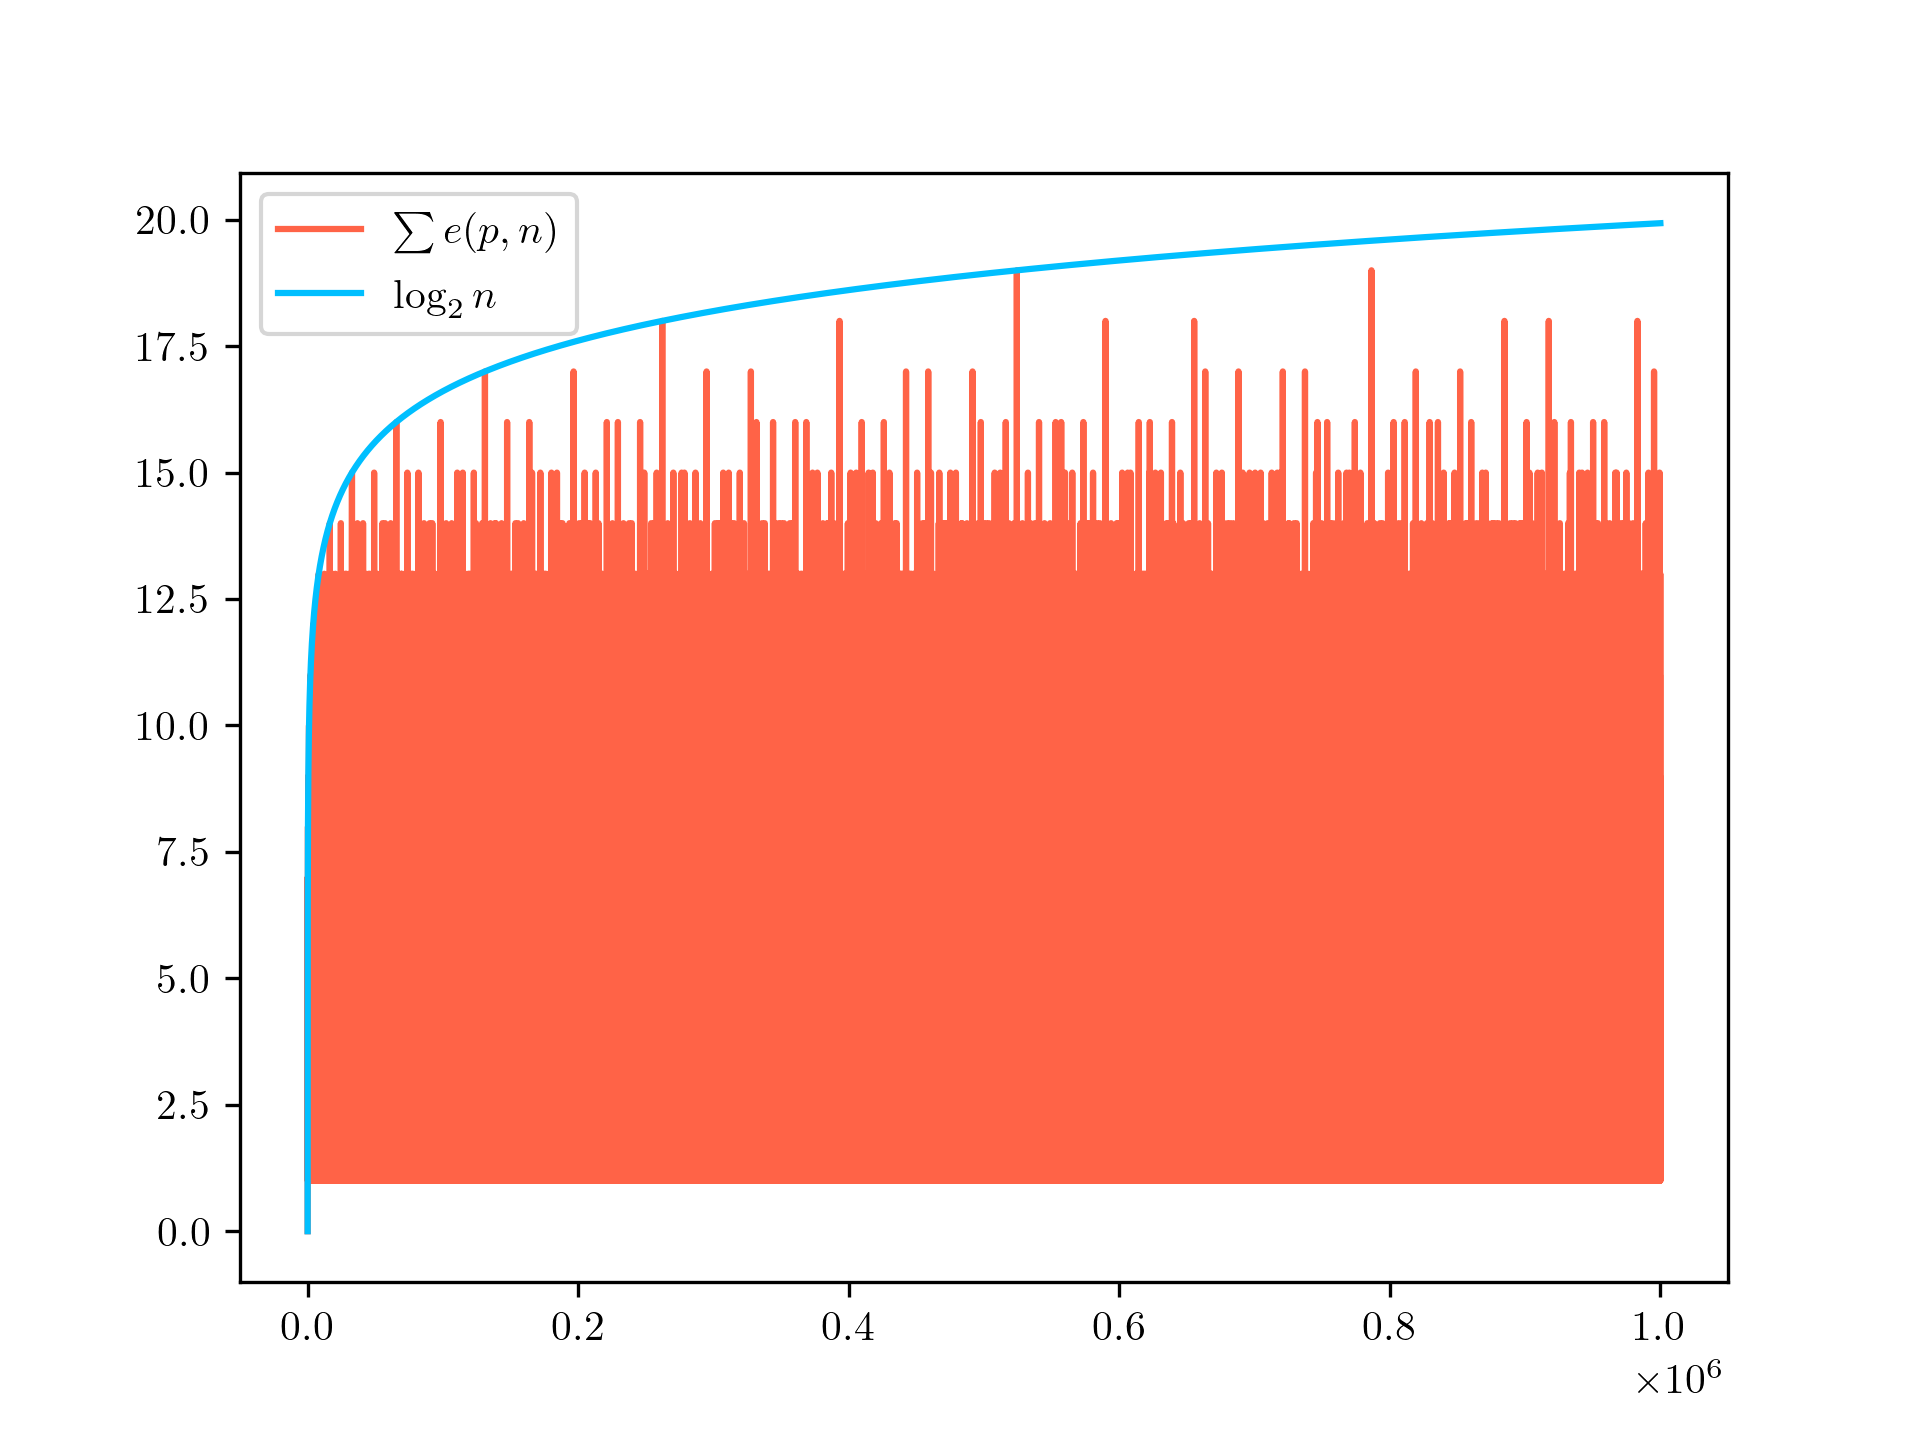
\includegraphics[keepaspectratio, scale=0.95]{img.png}
\end{figure}
\end{lem}

\vspace{1cm}

\begin{lem}\label{lem:dn}
\begin{equation}
d(n) = \prod e(p, n) + 1
\end{equation}
である。ただし $d(n)$ は $n$ の正の約数の個数である。
\end{lem}

\vspace{1cm}

\begin{alg} {\bf Osa\_k法による約数列挙} \upshape\\
\begin{lstlisting}
Class Osa_k():
    # Folding

    def d(self, n):
        min_factor = self.min_factor
        t = []
        tappend = t.append
        while n > 1:
            if t and t[-1][0] == min_factor[n]:
                t[-1][1] += 1
            else:
                tappend([min_factor[n], 1])
            n //= min_factor[n]
        res = 1
        for _, i in t:
            res *= i + 1
        return res

    def div(self, n):
        factors = self.__call__(n)
        res = {1, n}
        for i in range(1, len(factors)):
            for j in combinations(factors, i):
                tmp = 1
                for i in j:tmp *= i
                res |= {tmp}
        return res
\end{lstlisting}
\quad\\\itshape
補題 \ref{lem:dn} から明らかなように、約数個数は簡単に求めることができる。計算量 $O(\log n)$. 約数列挙は $O(\log n+d(n))$ ?ここでは最適化できていない。
\end{alg}



\vspace{1cm}

\begin{alg} {\bf 区間篩}\\\upshape
\begin{lstlisting}
def segmented_seive(l, r):
    rs = int(r ** .5) + 1
    # [2, √r]
    prime_small = [True] * rs
    prime_small[4::2] = [False] * (rs//2 - 1)
    # [l, r]
    prime = [True] * (r - l + 1)
    prime[l%2::2] = [False] * (r // 2 - (l - 1) // 2)
    for x in range(3, rs, 2):
        if prime_small[x]:
            for y in range(x*x, rs, x*2):
                prime_small[y] = False
            for z in range(((l + x - 1) // x | 1) * x, r, x*2):
                prime[z - l] = False
\end{lstlisting}
\quad\\
\end{alg}
前述したように区間 $[l, r]$ の素因数は $\sqrt{r}$ 以下であるから、これを利用して特定区間に対して篩をかけることができる。これを{\bf 区間篩}といい、 計算量は(おそらく)$O((r-l)\log\log r)$. ただし $\log\log\sqrt{r} = \log\log r + \log 2$ による。ただ上のコードは最適化されておらず $10^9$ を超えたあたりですぐに \lstinline{MemoryError}
を吐き(numba の jit である程度は回避可能)、逆に $10^7$ あたりであればエラトステネスの篩を普通に使って求めた方が明らかに高速なので、Pythonで使う限り出番があるかは微妙... numpy のベクトルを使えば最適化はできるかもしれない。もちろんこれを用いて素因数分解もできる。

\vspace{1cm}

\begin{exm}
$\displaystyle\sum_{K=1}^N Nd(N)$ を求めよ。$1\le N\le 10^7$.\upshape\ \ TL\ :\ 3\ sec\ \  \hspace{\fill} ABC172 D - Sum of Divisors\\
\begin{lstlisting}
# 2667 ms (PyPy)
P = Osa_k(10**7)
print(sum(i * P.d(i) for i in range(1, int(input()) + 1)))
\end{lstlisting}
\begin{lstlisting}
# 2096 ms (PyPy)
n = int(input())
F = [1] * -~n
for i in range(2, n + 1):
    for j in range(i, n + 1, i):
        F[j] += 1
print(sum(e * v for e, v in enumerate(F)))
\end{lstlisting}
\end{exm}

\vspace{1cm}

\begin{exm} 長さ $N$ の数列 $A$ が与えられるので、自然数 $i \le N$ であって $\forall j\in[1,N]_\ZZ, A_j \nmid A_i$ であるようなものの数を求めなさい。$1 \leq N \leq 2 \times 10^5, 1 \leq A_i \leq  10^6$\upshape \hspace{\fill} ABC170 D - Not Divisible\\
\begin{lstlisting}
# 1515 ms (PyPy)
from collections import Counter
n, *a = map(int, open(0).read().split())
b, c, P, cnt = set(a), Counter(a), Osa_k(10**6), 0
for i in b:
    if c[i] > 1:continue
    for d in P.div(i):
        if d != i and d in b:break
    else:
        cnt += 1
print(1 if n == 1 else cnt)
\end{lstlisting}
\begin{lstlisting}
# 665 ms (Python)
from collections import Counter
n, *A = map(int, open(0).read().split())
A.sort()
c, s = Counter(A), set()
M = max(A) + 1
ans = 0
for a in A:
    if a in s:
        continue
    ans += c[a] == 1
    for i in range(a, M, a):
        s.add(i)
print(ans)
\end{lstlisting}
\end{exm}

\vspace{1cm}

\begin{alg}{\bf ロー法による素因数分解}\upshape\\
\begin{lstlisting}
# O(⁴√n polylog(n))
def fast_prime_factorization(n):
    from subprocess import Popen, PIPE
    return [*map(int, Popen(["factor", str(n)], stdout=PIPE).communicate()[0].split()[1:])]

def fast_prime_factorization_many(lst):
    from subprocess import Popen, PIPE
    res = Popen(["factor"] + list(map(str, lst)), stdout=PIPE).communicate()[0].split(b"\n")[:-1]
    return [[*map(int, r.split()[1:])] for r in res]
\end{lstlisting}
\quad\\
bash には \lstinline{factor}
コマンドがあり、これを用いて比較的高速に素因数分解することができる。$O(\sqrt[4]{n}{\rm Li}(n))$ 程度(ただし ${\rm Li}(n)$ は多重対数 (polylog) 関数)。
\end{alg}

\vspace{1cm}

\begin{alg} {\bf 2015, Forisek らによる素数判定}\\\upshape
\begin{lstlisting}
import array
import bz2
import gzip
import base64
# depends on an env.
int32 = "l" if array.array("l").itemsize == 4 else "i"

bases = b'H4sIAEUphV0C/yy9X0zUabbv/dB0W...' # ...
bases = base64.b64decode(bases)
bases = gzip.decompress(bases)
bases = array.array(int32, bases)
assert len(bases) == 16384

def is_SPRP(n, a):
    if n==a: return True
    if n%a==0: return False
    d = m1 = n-1
    s = (d & -d).bit_length() - 1
    d >>= s
    cur = pow(a, d, n)
    if cur == 1: return True
    for _ in range(s):
        if cur == m1: return True
        cur = cur * cur % n
    return False

def is_prime(x):
    if x in {2, 3, 5, 7}: return True
    if x%2==0 or x%3==0 or x%5==0 or x%7==0: return False
    if x<121: return x>1
    if not is_SPRP(x, 2): return False
    h = ((x >> 32) ^ x) * 0x45d9f3b3335b369 & 0xffffffffffffffff
    h = ((h >> 32) ^ h) * 0x3335b36945d9f3b & 0xffffffffffffffff
    h = ((h >> 32) ^ h)
    b = bases[h & 16383]
    return is_SPRP(x, b&4095) and is_SPRP(x, b>>12)
\end{lstlisting}\itshape
\quad\\
Forisek and Jancina, 2015 を基に設計された素数判定アルゴリズムである(実装はLgeu氏のものによります)。小さな数字では効果は見られないが、\upshape 例えば超巨大な $23$ 桁程度の数も 41ms, メモリ 4KB と非常に軽動作で処理することができる。\lstinline{bases}
はあまりに長いので省略している。
\end{alg}

\section{テクニック}
\begin{alg}{\bf 二分探索} (Binary Search) とは、ソート済みのリストに対する検索を行うアルゴリズムであり、中央の値を見て、検索したい値との大小関係を用いて、検索したい値が中央の値の右にあるか、左にあるかを判断して、片側には存在しないことを確かめながら検索する手法。区間の範囲が半分半分に絞られていくイメージ。すなわち計算量 $O(\log N)$.\\\upshape
\begin{lstlisting}
from bisect import*
bisect_left(a, x, low = 0, high = len(a))
bisect_right(a, x, low = 0, high = len(a))
# bisect() = bisect_right()
# insort(a, x) := a.insert(bisect(a, x))
\end{lstlisting}
\quad\\ Python には標準ライブラリに \lstinline{bisect} モジュールがある。
\end{alg}

\vspace{1.5cm}

\begin{exm} $A_i < B_j < C_k$ となるような整数 $1\le i,j,k \le N$ の組の数を求めよ。$1 \le N \le 10^5$, $1 \le A_i, B_i, C_i, \le 10^9$. \upshape ABC077 C - Snuke Festival\\
\begin{lstlisting}
from bisect import*
(n,), a, b, c = [sorted(map(int, o.split())) for o in open(0)]
print(sum(bisect_left(a, B_j) * (n - bisect(c, B_j)) for B_j in b))
\end{lstlisting}\quad\\
解)$j$ を固定すると、二分探索によって $B_j$ より小さい / 大きい要素の数を数えることができるので、$j$ を全探索すれば良く、$O(N\log N)$ で解くことができた。
\end{exm}

\vspace{1cm}

\begin{exm} $L_i$ から三辺を選んで作れるような三角形の種類の数を求めよ。$3 \le N \le 2 \times 10^3$, $1 \leq L_i \leq 10^3$. \upshape ABC143 D - Triangles\\
\begin{lstlisting}
from bisect import*
n, *l = map(int, open(c:=0).read().split())
l.sort()
for i in range(n):
    for j in range(i+1, n):
        d = bisect_left(l, l[i] + l[j])
        c += max(0, d - j - 1)
print(c)
\end{lstlisting}\quad\\
解)$L$ をソートし、 $i < j < k$ かつ $L_k < L_i + L_j$ となるように選べば良い。 $O(N^2\log N)$.
\end{exm}

\vspace{1cm}

\begin{alg}{\bf 二分法} (Bisection method) では、単調増加関数 $f$ に対して二分探索をする。これに \lstinline{bisect} は対応していないので、自己実装する必要がある。
下のように半開区間 $(ng, ok]$ / $[ok, ng)$ で考える二分探索 / 二分法を提唱者 (@meguru\_comp) からめぐる二分探索という。二分探索は自明に計算量は $O(\log n)$. 二分法も $O(\log |ok-ng|)$ 程度。
\\\upshape
\begin{lstlisting}
def meg_bisect(ng, ok, func):
    while abs(ok - ng) > 1:
        mid = (ok + ng) // 2
        if func(mid):
            ok = mid
        else:
            ng = mid
    return ok
\end{lstlisting}
\end{alg}

\vspace{1cm}

\begin{exm} $d(N)\coloneqq N$ の十進表記桁数 とするとき、区間 $[1,10^9]$ にあるような整数 $N$ を買うのに必要な金額は $AN+Bd(N)$ 円である。$X$ 円で買える最大の整数はなにか。存在しない場合は $0$ とする。$1 \le A,B \le 10^9$, $1 \le X \le 10^{18}$.\ \upshape ABC146 C - Buy an Integer\\
\begin{lstlisting}
a, b, x = map(int, input().split())
print(meg_bisect(10**9 + 1, 0, lambda i:a * i + b * len(str(i)) <= x))
\end{lstlisting}
\end{exm}

\vspace{1cm}

\begin{exm} 長さ $A_i$ の丸太 $N$ 本を合計 $K$ 回まで切ったとき丸太の長さの最大値の最小値切り上げを求めよ。$1 \leq N \leq 2 \times 10^5$, $0 \leq K \leq 10^9$, $1 \leq A_i \leq 10^9$.\ \upshape ABC174 E - Logs\\
\begin{lstlisting}
n, k, *a = map(int, open(0).read().split())
print(meg_bisect(0, max(a), lambda x:sum(0--b // x - 1 for b in a) <= k))
\end{lstlisting}\quad\\
最大値の最小化は二分探索!典型!$x$ を最大値にするのに必要な切断回数は $\sum \lceil A_i / x \rceil - 1$ .
\end{exm}

\vspace{1cm}

\begin{exm}\upshape 赤い花 $R$ 本, 青い花 $B$ 本のうちいくつかを使って、それぞれ ($x$ 本, $1$ 本) で赤い花束、($1$ 本, $y$ 本) で青い花束を作れる。このとき、合計で花束は最大何本作れるか。 $1 \le R, B \le 10^{18}$, $2 \le x, y \leq 10^9$.\  ARC050 B - 花束\\
\begin{lstlisting}
R, B, x, y = map(int, open(0).read().split())
print(meg_bisect(min(R, B) + 1, 0, lambda k:(R - k) // (x - 1) + (B - k) // (y - 1) >= k))
\end{lstlisting}\quad\\
$k$ 本の花束を作るには赤青とも $k$ 本は必ず必要であり、それをまず最初に引いて考えると、作れる花束の数は $\left\lfloor\frac{R-k}{x-1}\right\rfloor + \left\lfloor\frac{B-k}{y-1}\right\rfloor$ であり、これが $k$ 本を超えていれば良い。解 $x$ がとりあえず存在すると仮定して Greedy に可能かを判定する問題として解くのは典型。
\end{exm}

\vspace{1cm}

\begin{exm}\upshape 最初高度 $H_i$ にある風船 $N$ 個について、競技開始 $0$ 秒後から $1$ 秒に $1$ 個の任意の風船を撃ち落とすことができるが、それぞれの風船は毎秒 $S_i$ の速度で上がっていく。それぞれの風船についてそれを撃ったときの高度がペナルティになるので、その最大値の最小値を求めよ。$1 \le N \le 10^5$, $1 \le H_i, S_i \leq 10^9$.\ \ TL\ :\ 5\ sec\ \ \  ABC023 D - 射撃王\\
\begin{lstlisting}
inf = 10**16    # max(H + N * S)
(n,), *d = [[*map(int, o.split())] for o in open(0)]
print(meg_bisect(0, inf, lambda x: all(l >= e for e, l in enumerate(sorted((x - h) // s for h, s in d)))))
\end{lstlisting}\quad\\
最大値を $x$ に保つには、それぞれの $i$ についてリミット $\left\lfloor\frac{x-H_i}{S_i}\right\rfloor$ 秒を記録し、ソートして厳しい順に Greedy に処理していって間に合うか試せば良い。計算量 $O(N\log\inf)$.
\end{exm}

\vspace{1cm}

\begin{exm}\upshape $f(t) \coloneqq At + B\sin(Ct\pi)$. $f(t)=100$ となるような 非負実数 $t$ をひとつ求めよ。誤差は $|f(t)-100|\le10^{-6}$ であれば認める。 $1 \le A,B,C \le 100$.\ ABC026 D - 高橋君ボール1号\\
\begin{lstlisting}
def meg_bisect_r(ng, ok, func, eps = 1e-9):
    while abs(ok - ng) > eps:
        mid = (ok + ng) / 2
    # folding...
from math import*
A, B, C = map(int, input().split())
f = lambda t:A * t + B * sin(C * t * pi)
print(meg_bisect_r(-1, 200, lambda t: f(t) >= 100, 1e-12))
\end{lstlisting}
\begin{lstlisting}
from scipy.optimize import*
print(newton(lambda t: f(t) - 100, 0))
\end{lstlisting}\quad\\
実数の二分法をするには、誤差を設定して行う。
\end{exm}

\vspace{1cm}

\begin{exm}\upshape 濃度 $p_i$ で $w_i$ グラムの食塩水 $N$ 個について、$K$ 個混ぜ合わせたときの濃度の最大値を求めよ。 $1 \le K,N \le 1000, 1\le w_i \le 10^9$.\ ABC034 D - 食塩水\\
\begin{lstlisting}
(n, k), *d = [[*map(int, o.split())] for o in open(0)]
print(meg_bisect_r(100.01, 0, lambda q: sum(sorted(w * (p - q) for w, p in d)[-k:]) >= 0))
\end{lstlisting}\quad\\
混ぜ合わせた後の食塩水の濃度が $q$ 以上、つまり $\displaystyle\frac{\sum w_ip_i}{\sum w_i} \le q$ となるには、$\sum w_ip_i - q \sum w_i \ge 0$ すなわち $\sum w_i(p_i-q)\ge 0$ ならばよい。
\end{exm}

\vspace{1cm}

\begin{alg}{\bf 三分探索} (Ternary Search) とは、高々極値が $1$ つであるような凸関数に対する三分割探索法。\\\upshape
\begin{lstlisting}
def trisect(func, left, right, eps = 1e-9):
    while abs(right - left) > eps:
    # for _ in [None] * limit:
        mid_l = (left * 2 + right) / 3
        mid_r = (left + right * 2) / 3
        if func(mid_l) < func(mid_r):
            right = mid_r
        else:
            left = mid_l
        return (right + left) / 2
\end{lstlisting}
\end{alg}

\vspace{1cm}

\begin{exm} ムーアの法則が正しいとすると、$x$ 年後にコンピュータの速度は $2^{x/1.5}$ 倍になる。現代で $P$ 年かかる計算は最小でいつ終わらせることができるか。すなわち、計算を始めるまでの時間とそこから計算にかかる時間の合計の最小値をもとめよ。$P\in(0,10^{18}]_\mathbb{R}$.\\\upshape
\begin{lstlisting}
P = float(input())
f = lambda x: x + P / pow(2, x / 1.5)
print(f(trisect(f, 0, 100)))
\end{lstlisting}\quad\\
$f(x)\coloneqq x + 2^{-x/1.5}P$ は凸関数である。三分探索で $\min f(x) = f({\rm argmax} f(x))$ と求める。
\end{exm}

\newpage

\begin{alg}{\bf 累積和} (accumulate) とは、事前に列 $A_i$ について\upshape $A'_i = \displaystyle\sum_{j=0}^{i-1} A_j$ ($A'_0 = 0$) となるようなリストを作っておくことで配列上の区間の総和を求めるクエリを $O(1)$ で処理する方法である。例えば $\displaystyle\sum_{k\in[i,j)} A_k = A'_j - A'_i$ と求めることができる。Python では \lstinline{itertools.accumulate} を用いれば良いが、$A'_0$ を含んでくれないので適宜調整する。
\end{alg}

\vspace{1cm}

\begin{exm} 長さ $N$ である数列 $A$ の {\bf 空でない連続する} 部分列であって、その総和が $0$ になるものの個数を求めよ。なお、列として同じでも位置が違うものは違う部分列とする。\upshape $1\le N\le 2\times 10^5$, $-10^9\le A_i\le10^9$.\ \ AGC023 A - Zero-Sum Ranges\\
\begin{lstlisting}
from itertools import*
from collections import*
*A, = accumulate(map(int, open(0).read().split()[1:]))
print(sum(k * (k - 1) // 2 for k in Counter([0] + A).values()))
\end{lstlisting}\quad\\
添字区間 $[i,j]$ での部分列の総和が $0$ になるとは、$A'_{j-1} = A'_i$ となることである。このような $(i,j)$ の選び方は、ある要素が数列 $A'_i$ に含まれる数を $k$ とすると $\sum_k{}_kC_2=\sum_kk(k-1)/2$ と求められる。
\end{exm}

\vspace{1cm}

\begin{exm} $Q$ 個のクエリで奇数 $l_i\le r_i$ が与えられるので、区間 $[l_i,r_i]$ 内で $x$ も $(x+1)/2$ も素数となるような奇数 $x$ の数を求めよ。$1\le N, l_i, r_i \le 10^5$.\ \upshape ABC084 D - 2017-like Number\\
\begin{lstlisting}
INF = 10**5 + 1
p, q = prime_checker(INF), [0] * INF
from itertools import*
for i in range(1, INF, 2):
    q[i] = p[i] * p[(i + 1)//2]
*q, = accumulate([0] + q)
for _ in [None] * int(input()):
    l, r = map(int, input().split())
    print(a[r + 1] - a[l])
\end{lstlisting}\quad\\
事前に配列 $p$ としてエラトステネスの篩を構成する。そして $q_i\coloneqq p_i \land p_{(i+1)/2}$ とすれば $q$ は条件を満たすか示す配列である。あとは累積和 $q'$ をとってクエリに回答する。
\end{exm}

\vspace{1cm}

\begin{exm} 数列 $A_i$ のうち、最大 $1$ つの要素を $[1,10^9]$ 内の整数に書き換えたとき、全体の最大公約数の最大値を求めよ。 $2\le N \le 10^5$, $1\le A_i \le 10^9$.\ \upshape ABC125 C - GCD on Blackboard\\
\begin{lstlisting}
from itertools import*
from math import*
n, *a = map(int, open(0).read().split())
*f, = accumulate([0] + a, gcd)
*b, = accumulate(a[::-1], gcd)
print(max(gcd(s, t) for s, t in zip(f, b[::-1])))
\end{lstlisting}\quad\\
まず、違う整数に置き換えたところで最大公約数が増えることはなく、置き換える動作は取り除く動作としてよい。\lstinline{itertools.accumulate} は第 $2$ 引数を取ることができ、$\gcd$ は結合則が成り立つことから累積でいいとわかる。自分より左の区間と右の区間が必要なので逆からの累積もとる。
\end{exm}

\newpage

\begin{alg} {\bf 2次元累積和} 累積和は同様に $2$ 次元にも拡張できる。\\\upshape
\begin{lstlisting}
# [x1, x2) × [y1, y2)
def ac2(s:list, x1, x2, y1, y2):
    return s[x2][y2] - s[x1][y2] - s[x2][y1] + s[x1][y1]
\end{lstlisting}\
\end{alg}

\vspace{1cm}

\begin{exm} $N\times N$ のたこ焼き器があり、それぞれの場所に美味しさ $D_{ij}$ が決まっている。いま、$Q$ 人の店員がやってきて、長方形の形をした領域で最大 $P_k$ このたこ焼きを焼くとき、それぞれの店員について美味しさの総和の最大値を求めよ。$1\le N \le 50$, $1\le D_{ik}\le 100$, $1\le Q,P_k \le N^2$.\upshape\ TL:5sec ABC005 D - おいしいたこ焼きの焼き方\\
\begin{lstlisting}
import numpy as np
from itertools import*
n = int(input())
D = np.array([[0]*-~n]+[[0]+[*map(int, input().split())] for _ in [0]*n])
D = np.cumsum(D, axis = 0)
D = np.cumsum(D, axis = 1)
dp = [0] * (n * n + 1)
for x1 in range(n):
    for i in range(1, n - x1 + 1):
        x2 = x1 + i
        for y1 in range(n):
            for j in range(1, n - y1 + 1):
                y2 = y1 + j
                dp[i*j] = max(dp[i*j], ac2(D, x1, x2, y1, y2))
*dp, = accumulate(dp, max)
for _ in [None] * int(input()):
    print(dp[int(input())])
\end{lstlisting}
\quad\\
\lstinline{np.cumsum}
を使うと実装が楽。\lstinline{itertools.accumulate(dp, max)}
は「今までで出た最大値」を取る動作になっている。$O(N^4)$.
\end{exm}

\vspace{1cm}

\begin{alg} {\bf imos法} は、配列上の特定区間 $[l, r]$ に $v$ 加算するクエリを、 $0$ で初期化した配列に対し $l$ に $v$ 加算、$r + 1$ に $v$ 減算しての操作を繰り返し最後に累積和を取ることで処理する方法である。@imos 氏が京都大学院での修士論文で取りまとめたことからこの名がある。\\\upshape
\begin{lstlisting}
from itertools import*
class Imos:
    def __init__(self, n):
        self.B = [0] * n
        self.n = n

    def __call__(self, l, r, v = 1):
        l, r = max(l, 0), min(r, self.n - 1)
        self.B[l] += v
        if r + 1 != self.n:
            self.B[r + 1] -= v

    def out(self):
        *res, = accumulate(self.B)
        # self.__init__(self.n)
        return res
\end{lstlisting}
\end{alg}
\vspace{1.5cm}
\newpage
\begin{exm} 黒面に $0$、白面に $1$ がかかれた $N$ 個のオセロが最初全て黒面を表に一列に並べられている。$Q$ 回の操作で $[l_i,r_i]$ 番目全てを裏返すことを繰り返すとき最終盤面を出力せよ。$1\le l_i\le r_i \le N,Q\le 2\times10^5$.\ \upshape\ ABC035 C - オセロ\\
\begin{lstlisting}
(n, q), *Q = [[*map(int, o.split())] for o in open(0)]
imos = Imos(n + 1)
for l, r in Q:
    imos(l, r)
print(*[i%2 for i in imos.out()[1:]], sep = "")
\end{lstlisting}\quad\\
加算する操作として最後に $\hspace{-0.6mm}\mod 2$ を取ればよい。
\end{exm}

\vspace{3cm}

\begin{exm}
濃さ $0$ から $10^6$ までの濃さの絵具がそれぞれ売られている。$n$ 人の顧客がそれぞれ $[a_i,b_i]$ 内の濃さの絵具なら購入するとき、最も多くの顧客に買われる絵具は何人に買われるだろうか。 $1\le n \le 10^5$, $0\le a_i\le b_i\le 10^6$.\ \ \upshape TL:3sec ABC014 C - AtColor\\
\begin{lstlisting}
imos = Imos(10**6 + 1)
_, *q = [[*map(int, o.split())] for o in open(0)]
for l, r in q:
    imos(l, r)
print(max(imos.out()))
\end{lstlisting}
\end{exm}

\newpage

\begin{exm} $C$ 個のチャンネルがあるテレビで $N$ 個のテレビ番組を録画したい。番組 $i$ は時刻 $[s_i,t_i)$ に $c_i$ 番目のチャンネルで放送されている。ある録画機で $[s,t)$ の番組を予約すると $[s-0.5,t)$ の間 {\bf 他のチャンネル} の録画には使えないので、全て録画するのに必要な録画機の最小個数を求めよ。$1\le N\le 10^5$, $1\le c_i\le C\le 30$, $1\le s_i < t_i\le 10^5$.\upshape ABC080 D - Recording\\
\begin{lstlisting}
from collections import defaultdict
d = defaultdict(list)
imos = Imos(10 ** 5 + 1)

(N, C), *D = [[*map(int, o.split())] for o in open(0)]
for s, t, c in D:
    d[c] += (s, t),
for p in d.values():
    p.sort()
    ps, pt = p[0]
    for s, t in p[1:] + [[0,0]]:
        if pt == s:
            pt = t
        else:
            imos(ps - 1, pt - 1)
            ps, pt = s, t
print(max(imos.out()))
\end{lstlisting}
\quad\\
ソートし、同じチャンネルで番組が続くような場合は結合して一つの番組として扱うような実装にする。$[s-0.5,t)$ を占領するとは $[s-1,t-1]$ を占領するとして問題ないことがわかる。
\end{exm}

\vspace{1cm}\newpage

\begin{exm}
$N$ 個の電球が数直線上にあり、電球 $i$ は座標 $(i)$ にある。電球 $x$ の光の強さが $d$ であるとき、その電球は $[x-d-0.5,x+d+0.5]$ を照らす。初めの光の強さは $A_i$ で与えられる。今、「それぞれの電球について電球 $i$ の強さを座標 $(i)$ を照らしている電球の数に置き換える」という操作を $K$ 回繰り返すとき、最終的な各電球の光の強さを求めよ。$1\le N,K\le 2\times10^5$, $0\le A_i\le N$ \quad\upshape 東京海上日動2020 C - Lamps\\
\begin{lstlisting}
from itertools import*
n, k, *A = map(int, open(0).read().split())
for _ in [0] * min(k, 41):
    imos = Imos(n)
    for i, a in enumerate(A):
        imos(i - a, i + a)
    A = imos.out()
print(*A)
\end{lstlisting}\quad\\
$K$ が十分大きいとき、$\log N$ 回程度で数列は収束し $A'_i = N$ のような配列になることがわかる。最悪ケースで試しても実際 $41$ 回で終了するし、全ての要素が $N$ になる時に打ち切れば十分である。計算量は $O(N \min(K, \log N))$ .
\end{exm}

\vspace{1cm}

\begin{exm} $M$ 個の区間が与えられ、$i$ 番目の区間では $N$ 個の教室のうち $[s_i,t_i]$ の教室を掃除する。この中で、その区間を抜いても全教室を掃除できるようなものの総数とその番号 $i$ を順に出力せよ。$1\le s_i \le t_i\le N \le 3\times10^5$, $1\le M\le 10^5$\quad \upshape ARC045 B - ドキドキデート大作戦高橋君\\
\begin{lstlisting}
(n, m), *q = [[*map(int, o.split())] for o in open(0)]
imos = Imos(n + 2)
for s, t in q:
    imos(s, t)
*c, = accumulate([0] + [i > 1 for i in imos.out()])
ans = []
for e, (s, t) in enumerate(q, 1):
    if c[t + 1] - c[s] == t - s + 1:
        ans += e,
print(len(ans))
for i in ans:
    print(i)
\end{lstlisting}
\quad\\
imos法の配列のそれぞれの要素について重複しているか $?(i > 1)$ を判別しそれで累積和 $c$ を取る。区間 $[s,t]$ を抜いてもいいとは $c_{t+1} - c_s = t - s + 1$ となることである。
\end{exm}

\vspace{1cm}

\begin{exm}
$N$ 個の遺跡と $M$ 種類の宝石がある。遺跡 $i$ では、得点 $s_i$ 点と $[l_i,r_i]$ の宝石を獲得する。違う遺跡をいくつか探索したとき、得点の最大値はいくらか。ただし{\bf 全種類の宝石を集めてはならない}。$1\le N,M\le 10^5$, $1\le s_i\le 5000$, $1\le l_i \le r_i \le M$. \quad\upshape ABC017 C - ハイスコア\\
\begin{lstlisting}
(n, m), *D = [[*map(int, o.split())] for o in open(0)]
imos = Imos(m + 1)
for l, r, s in D:
    imos(l, r, s)
print(sum(d[2] for d in D) - min(imos.out()[1:]))
\end{lstlisting}\quad\\
それぞれの宝石について、「その宝石を集めないとしたとき、{\bf 全ての遺跡を訪れたときからの得点減少分}」をimos法で記録する。これは $[l,r]$ に $s$ 加算する操作で良い。
\end{exm}

\newpage

\begin{exm} ある日の雨の降り始めた時刻 $S_i$ と降り終えた時間 $E_i$ の組を書いた降水メモが $N$ 個ある。まず雨の降り始め・降り終わりをそれぞれ直前・直後の $5$ 分単位の時刻に丸める。この丸め終えたあとのメモにおいて、時間の重複があった場合それをつなげて改めて出力せよ。$1\le N\le 30000$, $00:00\le S_i\le E_i \le 24:00$\\\upshape
\begin{lstlisting}
def I(t: "hhmm") -> "min.":
    h, m = map(int, (t[:2], t[2:]))
    return h * 60 + m

def O(t: "min.") -> "hhmm":
    h, m = divmod(t, 60)
    return str(h).zfill(2) + str(m).zfill(2)

def round5(a, b):
    return a // 5 * 5, 0--b // 5 * 5

r, imos = range(24 * 60 + 1), Imos(24 * 60 + 1)
for i in range(int(input())):
    imos(*round5(*map(I, input().split("-"))))

D = imos.out()
S = [[*l] for k, l in groupby(r, key = lambda i: D[i] > 0) if k]
for s, *_, e in S:
    print(f"{O(s)}-{O(e)}")
\end{lstlisting}\quad\\
いわゆる「やるだけ」問題だが、imos法を使うとわかりやすくかつ高速に処理することができる。
\end{exm}
\newpage
\section{データ構造}

\begin{alg} {\bf 素集合データ構造} (Disjoint-set Data Structure) あるいは {\bf UnionFind木} とは、互いに素な集合群に対するデータ構造であり、Union : 2つの集合を1つに統合する 及び Find : 要素がどの集合に属しているか求める の二種類の操作ができるものをいう。\\\upshape
\begin{lstlisting}
class UnionFind():
    def __init__(self, n):
        self.n = n
        self.parents = [-1] * n

    def find(self, x):
        if self.parents[x] < 0:
            return x
        else:
            self.parents[x] = self.find(self.parents[x])
            return self.parents[x]

    def union(self, x, y):
        x = self.find(x)
        y = self.find(y)
        if x == y:
            return
        if self.parents[x] > self.parents[y]:
            x, y = y, x
        self.parents[x] += self.parents[y]
        self.parents[y] = x

    def size(self, x):
        return -self.parents[self.find(x)]

    def same(self, x, y):
        return self.find(x) == self.find(y)

    def members(self, x):
        root = self.find(x)
        return [i for i in range(self.n) if self.find(i) == root]

    def roots(self):
        return [i for i, x in enumerate(self.parents) if x < 0]

    def group_count(self):
        return len(self.roots())
\end{lstlisting}\quad\\
具体的には ${\rm Union}(x,y)$ で $x$ が含まれている集合と $y$ が含まれている集合を結合し、 ${\rm Find}(x)$ で $x$ の根番号を求める。この実装では計算量を落とす (Union by Rank) ために根の親の値に要素数を負の値で格納している。サイズやランクをリストで保持する実装が必要なくなっている。さらに \lstinline{find} では経路圧縮 (Path Compression) というテクニックを使っている。調べた要素の親を根に変更しつなぎ直すことで深い形状を解消している。これらのテクニックを落とすことでクエリ計算量を $O(\alpha(n))$ と実質定数にできる。
\end{alg}

\vspace{1cm}

\begin{defi} アッカーマン関数 $A_k(n):\mathbb{R}\rightarrow\mathbb{R}$ を以下のように再帰的に定義する。
\begin{align}
A_k (0) &= k + 1 \\
A_0 (n) &= A_1(n - 1) \\
{\rm otherwise:\quad}A_k (n) &= A_{A_{k - 1}(n)}(n - 1)
\end{align}
\end{defi}

\vspace{1cm}

\begin{defi} $\alpha(n)$ はアッカーマン関数の逆関数である。
\begin{align}
\alpha(n) = A_k^{-1}(m)
\end{align}
$A_k(n)$ は $n\ge 4$ において非常に大きく増加する関数であり、その逆関数である $\alpha(n)$ は例えば $k=2$ のとき $\alpha(2^{65536}-3)=4$. ここで $2^{65536}>> 10^{2\times 10^5}$ であるから、実質十分小さい定数とみなして良いといえる。クエリの計算量が $O(\alpha(n))$ である証明は非常に煩雑なので省略する。
\end{defi}
\newpage

\begin{defi}
集合 $X$ のある部分集合族 $\mathscr{F}$ について、$\mathscr{F}$ のどの要素においても $F\in\mathscr{F}$ が真部分集合でないとき、$F$ は $\mathscr{F}$ について極大な部分集合であるという。
\end{defi}

\vspace{1cm}

\begin{defi}
任意の2頂点間に何らかの経路が存在するグラフのことを {\bf 連結グラフ} (connected graph) という。部分グラフのうち連結グラフであるようなものの集合族において極大で連結な部分グラフを、{\bf 連結成分} (connected component) という。
\end{defi}

\vspace{1cm}

\begin{exm}自己ループと二重辺を含まない $N$ 頂点 $M$ 辺の無向連結グラフが与えられる。$i$ 番目の辺は頂点 $a_i,b_i$ を結んでいる。それを取り除いたときグラフ全体が非連結になるような辺のことを橋と呼ぶ。 $M$ 本のうち橋の数を求めよ。$2\le N \le 50$, $N-1\le M \le \min(n(n-1)/2, 50)$, $1\le a_i < b_i \le N$.\quad\upshape ABC075 C - Bridge\\
\begin{lstlisting}
(n, m), *q = [[*map(int, o.split())] for o in open(0)]
uf, c = UnionFind(n), 0
for i in range(m):
    for j, (a, b) in enumerate(q):
        if i == j: continue
        uf.union(a - 1, b - 1)
    c += UF.group_count() > 1
print(c)
\end{lstlisting}\quad\\
制約が小さいので実際に構築し全ての頂点が同じ集合に属しているか確認すれば良い。
\end{exm}

\newpage

\begin{defi}
グラフの頂点 $v$ に接続する辺の本数を $v$ の次数 (degree) という。また、閉路を含まないグラフを{\bf 森} (forest) といい、連結な森を {\bf 木} (tree) と呼ぶ。
\end{defi}

\SS

\begin{thm}
$T$ が $n$ 頂点の木ならば、$T$ は $n − 1$ 本の辺をもつ。
\begin{proof} (証明) $n=1$ のとき明らか。以下 $n\ge 2$ における帰納法による。頂点数が $m$
以下まで仮定。$T$ の頂点数を $m + 1$ とする。$T$ から次数 $1$ の頂点とその頂点に接続する辺を除去して得られる木を $T'$ とすると、$T'$ の頂点数は $m$. 帰納法の仮定より、$T'$ の辺数は $m − 1$. $T'$ の構成方法より、$T$ の辺数は $T'$ より $1$ つだけ大きい。したがって、$T$ の辺数は $m$ である。

\end{proof}
\end{thm}
\begin{exm}
自己ループと二重辺を含まない $N$ 頂点 $M$ 辺の無向グラフが与えられる。 $i$ 番目の辺は頂点 $u_i,v_i$ を結んでいる。 このグラフの連結成分のうち木であるようなものの個数を求めよ。$2\le N \le 100$, $1\le M \le N(N-1)/2$, $1\le u_i < v_i \le N$.\quad\upshape ARC037 B - バウムテスト\\
\begin{lstlisting}
(n, _), *q = [[*map(int, o.split())] for o in open(0)]
uf = UnionFind(n)
for u, v in q:
    uf.union(u - 1, v - 1)

edge = [0] * n
for u, _ in uv:
    edge[uf.find(u)] += 1

node = [0] * n
for i in range(n):
    node[uf.find(i)] += 1

print(sum(node[i] == edge[i] + 1 for i in range(n)))
\end{lstlisting}
\end{exm}

\newpage

\begin{exm} ある街には $N$ 個の交差点と $M$ 本の道路があり、$i$ 番目の道路は交差点 $a_i,b_i$ を結んでいる。どの交差点からも道路で別のどの交差点にも行けるようにするには最小で何本の道路を建設する必要があるか。$1 \le N \le 10^5$, $0 \le M \le 10^5$, $1 \le a_i < b_i \le N$\upshape\quad ARC032 B - 道路工事\\
\begin{lstlisting}[frame = none]
(n, m), *q = [[*map(int, o.split())] for o in open(0)]
uf = UnionFind(n)
for a, b in q:
    uf.union(a - 1, b - 1)
print(uf.group_count() - 1)
\end{lstlisting}
\end{exm}

\SS

\begin{exm}\upshape
とあるSNSでは、$A_i$ と $B_i$ $(1\le i\le M)$ の間に友達関係があり、$C_i$ と $D_i$ $(1\le i\le K)$の間にブロック関係がある。異なる人の組 $(a,b)$ であって、友達関係でもブロック関係でもなく、数列 $c_i$ であって( $c_0 = a \land c_L = b \land \forall i \in [0,L), c_i$ と $c_{i+1}$ は友達関係である)を満たすようなものが存在しているとき、人 $a,b$ は友達候補であるとする。それぞれの人に対し友達候補の数を求めよ。$2\le N\le 10^5$, $0\le M,K\le 10^5$.\quad ABC157 D - Friend Suggestions\\
\begin{lstlisting}[frame = none]
(n, m, k), *q = [[*map(int, o.split())] for o in open(0)]
UF, non_cand = UnionFind(n), [1] * n
for a, b in q[:m]:
    a -= 1; b -= 1
    UF.union(a, b)
    non_cand[a] += 1; non_cand[b] += 1
for c, d in q[m:]:
    c -= 1; d -= 1
    if UF.same(c, d):
        non_cand[c] += 1; non_cand[d] += 1
print(*[UF.size(i) - non_cand[i] for i in range(n)])
\end{lstlisting}\quad\\
友達関係でUnionFindを構築する。それぞれの人に対して属する連結成分のサイズを求め、非候補[自分($1$ で初期化)、友達関係、同じ連結成分に属しブロック関係、の合計]を引けば良い。
\end{exm}

\newpage

\begin{defi} 木の末端の辺を葉という。グラフ $G(V,E)$ の頂点集合 $V$ と辺集合の部分集合 $T\subseteq E$ からなる $G'(V,T)$ が木のとき、$G'$ は $G$ の{\bf 全域木} であるという。
\end{defi}

\SS

\begin{exm} $N$ 以下の正整数を並び替えた数列 $p_1,\ldots,p_N$ と $N$ 以下の正整数の組 $(x_i,y_i)$ が $M$ 個与えられる。「任意の $j$ を選び $p_{x_j},p_{y_j}$ をスワップする」動作を任意の回数行えるとき、最終的に $p_i=i$ となる $i$ の最大数を求めよ。 $2\le N\le 10^5$, $1\le M\le 10^5$. \quad\upshape ARC 097 D - Equals\\
\begin{lstlisting}
(n, m), p, *q = [list(map(int, o.split())) for o in open(0)]
UF = UnionFind(n + 1)
for a, b in q:
    UF.union(a, b)
print(sum(UF.same(p[i], i + 1) for i in range(n)))
\end{lstlisting}\quad\\
頂点集合 $V=[1,N]\cap\ZZ$, 辺集合 $E=\left\{(x_i,y_i)\mid1\le i\le M\right\}$ から成るグラフ $G(V,E)$ を考える。$G$ の連結成分の集合 $G'={g_k}$ に対して $\exists g_k\in G', (p_i,i) \in g_k^2$ ならば $p_i=i$ とできる(証明は以下)。また逆は明らかなので、UnionFind を構築しその数を数えれば良い。
\begin{proof}
各 $k$ に対して、全単射 $f:g_k \rightarrow \left\{p_i\mid i \in g_k \right\}$ であって
\begin{equation}
\exists g_k\in G', (p_i,i) \in g_k^2 \Longleftrightarrow f(i)=i
\end{equation}
と成るようなものが存在し、うまく全域木をとり葉 $i$ に $f(i)$ をおく操作を繰り返せばよい、
\end{proof}
\end{exm}

\SS

\begin{exm} $N$ 枚のカードについて、$i$ 番目に書かれた数字は $A_i$ で、$1$ か $2$ のどちらかである。今、$M$ 個の情報が与えられ、$A_{X_i}+A_{Y_i}+Z_i \in 2\ZZ$ である。少なくともいくつ $A_i$ の値を知れば全ての $A_i$ の値がわかるか。$2\le N\le 10^5$, $1\le M\le 10^5$, $1\le Z_i\le 100$. \quad\upshape ABC126 E - 1 or 2
\begin{lstlisting}
(n, m), *q = [list(map(int, o.split())) for o in open(0)]
UF = UnionFind(n)
for x, y, _ in q:
    UF.union(x - 1, y - 1)
print(UF.group_count())
\end{lstlisting}\quad\\
$Z_i$ の偶奇によって、$A_{X_i},A_{Y_i}$ は偶奇が同じ / 異なるという情報を得る。数字は $1$ か $2$ のみだから、$X_i,Y_i$ を繋ぐ UnionFind の連結成分数だけわかれば最終的に連鎖的に値は決定する。
\end{exm}

\SS

\begin{exm} $N$ 個の島および島 $A_i,B_i$ を結ぶ全て異なる橋が $M$ 本ある。はじめどの $2$ 島についても何らかの経路が存在するが、橋は $1$ 番目から順に全て崩落する。行き来できない島の組 $a<b$ の数を不便さと呼ぶとき、$i$ 番目の橋が崩落した直後の不便さを答えよ。$2\le N\le 10^5$, $1\le M\le 10^5$\quad\upshape ABC120 D - Decayed Bridges\\
\begin{lstlisting}
(n, m), *q = [map(int, o.split()) for o in open(0)]
UF = UnionFind(n)
conv = [n * (n - 1) // 2]
for a, b in q[::-1]:
    a -= 1; b -= 1
    if UF.same(a, b):
        conv += conv[-1],
    else:
        conv += conv[-1] - UF.size(a) * UF.size(b),
    UF.union(a, b)
assert conv[-1] == 0
for i in conv[-2::-1]: print(i)
\end{lstlisting}\quad\\
クエリを先読みして逆順に処理し不便さを減らしていくようにすれば求めることができる。
\end{exm}

\newpage

\begin{exm} ある星には $M$ 種類の言語がある。$N$ 人の人がいて、それぞれ $K_i$ 種類の言語 $L_{i1},\ldots L_{iK_i}$ を話すことができる。ある $2$ 人はともに話すことの出来る言語が存在する、あるいはともにコミュニケーションをとることができる人が存在するとき、コミュニケーションをとることができる。全ての人が他の全ての人とコミュニケーションをとれるか判定せよ。$2\le N\le 10^5$, $1\le M\le 10^5$, $\sum K_i \le 10^5$.\quad\upshape CODE FESTIVAL '16 Final C - Interpretation\\
\begin{lstlisting}
(n, m), *LL = [[*map(int, o.split())] for o in open(0)]
UF = UnionFind(n + m)
for e, (k, *L) in enumerate(LL):
    for l in L:
        UF.union(e, l + n - 1)
print(len([*filter(lambda i: i < n, UF.roots())]) == 1 and "YES" or "NO")
\end{lstlisting}\quad\\
人を $[0,N)$ 、言語を $[N,N+M)$ で管理し、それぞれの人について話せる言語に辺を貼り、連結成分の数を数えれば良い。ただし、番号が $N$ 未満の根に絞らないと言語が残っていても判定されてしまうので注意。
\end{exm}

\SS

\begin{exm} ある国には $N$ 個の都市と $M$ 本の道路があり、$i$ 本目の道路は都市 $a_i, b_i$ を結び $y_i$ 年に作られた。$Q$ 人の住民について、$j$ 人目の住民は都市 $v_j$ に住んでおり $w_j$ 年以前に作られた道路を通らない。それぞれの住民に対して行くことができる都市の数を求めよ。$1\le N,Q\le 10^5$, $0\le N\le 10^5$, $1\le y_i\le 2\times 10^5$, $0\le w_i\le 2\times 10^5$.\quad\upshape ABC 040 D - 道路の老朽化対策について\\
\begin{lstlisting}
(n, m), *d = [[*map(int, o.split())] for o in open(0)]
I, q, J = d[:m], int(*d[m]), d[m + 1:]
data = []
for a, b, y in I:
    data += [-y, 1, a, b],
for e, (v, w) in enumerate(J):
    data += [-w, 0, e, v],
data.sort()

UF, ans = UnionFind(n + 1), [0] * q
for _, F, c, d in data:
    if F:
        UF.union(c, d)
    else:
        ans[c] = UF.size(d)

for s in ans:
    print(s)
\end{lstlisting}\quad\\
年の大きい方から処理していけばよい。なお、同じ年の中では住民クエリを先に処理する必要があることに注意。
\end{exm}

\SS

\begin{exm}先頭が $0$ でない $N$ 桁の整数を $2$ 回メモしたが、一部字が汚くアルファベットに見えている。同じアルファベットは同じ数字を表すとするとき(逆は必ずしも成り立たない)、最大で何種類の数が考えられるか。$1\le N\le 18$.\upshape\quad ARC027 B - 大事な数なのでZ回書きまLた。\\
\begin{lstlisting}
# print(ord("A")) -> 65
code = lambda char: ord(char) - 55 if char.isalpha() else int(char)

n = int(input())
*s1, = map(code, input())
*s2, = map(code, input())

UF = Un1onF1nd(36)
for s, t in zip(s1, s2):
    UF.un1on(s, t)

ans = 1
used = set()
for e, s in enumerate(s1):
    if any(UF.same(i, s) for i in range(10)) or (t := UF.f1nd(s)) in used:
        continue
    used |= {t}
    ans *= 10 - (e == 0)
print(ans)
\end{lstlisting}\quad\\
$s_{1i},s_{2i}$ を結んで得られるグラフの連結成分のうち数字が含まれているものは確定する。そうでないとき、$10$ 通りの可能性がある。ただし、先頭には $0$ は使えないので、それを考慮して前から見ていきすでにチェックしたルートはパスするようにすればよい。
\end{exm}

\SS

\begin{exm} $N$ 頂点 $M$ 辺の森が与えられる。頂点は $\bm{0{\rm -indexed}}$ \upshape で、辺は頂点 $x_i,y_i$ を結ぶ。各頂点には $a_i$ という値が決まっている。今、この森にいくつかの辺を張って木にすることを考える。ただし、頂点 $i,j$ を結ぶときコスト $a_i+a_j$ がかかり、さらに頂点は{\bf 一度しか選択できない}。 コストを最小化せよ。木にできないときは \lstinline{'Impossible'} と出力せよ。
$1\le N\le 10^5$, $0\le M\le N-1$, $1\le a_i\le 10^9$.\quad APC001 D - Forest\\
\begin{lstlisting}
(n, m), a, *q = [[*map(int, o.split())] for o in open(0)]
UF = UnionFind(n)
k = (n - m - 1) * 2
if k > n: exit(print("Impossible"))
if not k: exit(print(0))

for c, f in q:
    UF.union(c, f)

from collections import*
d = defaultdict(list)
for e, i in enumerate(a):
    d[UF.find(e)] += i,

ans, b = 0, []
for r, p in d.items():
    p.sort()
    ans += p.pop(0)
    b += p
    k -= 1
b.sort()
print(ans + sum(b[:k]))
\end{lstlisting}\quad\\
$N-1$ 辺にするのが目標である。よって、はる辺数は $N-M-1$ 本。必要な次数の合計は $K=2(N-M-1)$ 本だが、同じ頂点には二度とはれないことから少なくとも $K$ 頂点が必要になる。$K > N$ なら不可能で、そうでなければ構築可能なことがわかる。さらに、それぞれの連結成分に対して少なくとも $1$ つの頂点を選ぶ必要があるが、その残りはどの連結成分から選んでも構築方法が存在するとわかる。よって、まず全ての連結成分からコスト最小のものを選び、残りは全体の小さい順から選んでいけばよい。
\end{exm}

\SS

\begin{defi}
グラフ $G(V,E)$ において、頂点集合 $V$ を $2$ つの部分集合 $V_1,V_2$ に分割して各集合内の頂点同士の間には辺が無いようにできるとき、$G$ は {\bf 2部グラフ} (Bipartite Graph) であるといい、$G(V_1+V_2,E)$ などとかく。またこのとき、任意の $(u,v)\in V_1V_2$ について辺 $(u,v)$ が存在するとき、$G$ は {\bf 完全2部グラフ} (Complete Bipartite Graph) であるという。
\end{defi}

\SS

\begin{cor}
完全2部グラフ $G(V_1+V_2,E)$ において、辺の数は $|V_1||V_2|$ である。
\end{cor}

\SS

\begin{exm} $xy$ 座標平面上の第一象限に点 $(x_i,y_i)$ が重複なく $N$ 個ある。$(a, b), (a, d), (c, b), (c, d)$ のうち $3$ 箇所に点があるような整数 $a\ne c, b\ne d$ を選び、残りの $1$ 箇所に点を追加するという操作を行える限り繰り返す。この操作は有限回しか行えないことが証明できるが、操作回数の最大値はいくらか。$1\le N,x_i,y_i\le 10^5$. \upshape\quad ABC131 F - Must Be Rectangular!\\
\begin{lstlisting}
(n,), *q = [[*map(int, o.split())] for o in open(0)]
MAX = 10 ** 5 + 1
UF = UnionFind(2 * MAX)
for x, y in q:
    UF.union(x, y + MAX)
cnt_x = [0] * (2 * MAX)
cnt_y = cnt_x[:]
for i in range(MAX):
    cnt_x[UF.find(i)] += 1
    cnt_y[UF.find(i + MAX)] += 1
print(sum(X * Y for X, Y in zip(cnt_x, cnt_y)) - n)
\end{lstlisting}\quad\\
まず、2部グラフ $G(X+Y,E)$ を考えていくと、連結成分ごとに分解できる。ここで $X,Y$ はそれぞれ $x,y$ 座標の集合で、 $E$ は与えられた点の座標組である(座標平面を2部グラフとみなすのは典型)。そこで、この操作はそれぞれの連結成分について完全2部グラフになるまで行うことができるとわかる。よって、答えは $\sum |X||Y| - N$ である。
\end{exm}

\SS

\begin{exm} $N$ 個の駐車スペースと駐車スペース $u_i,v_i$ を結ぶ $M$ 本の道がある駐車場に、$N$ 人の人が順にやってくる。$i$ 番目の人は、駐車場の入り口から空いている駐車場と道を通って駐車スペース $i$ に車を駐めようとするが、たどり着くことができないときは帰ってしまう。駐車スペース $S$ が駐車場の入り口と繋がっているとき、駐車場に駐めることができる人の番号を順に出力せよ。$1\le N,M\le 2\times 10^5$.\quad\upshape ARC056 B - 駐車場\\
\begin{lstlisting}
(n, m, s), *q = [[*map(int, o.split())] for o in open(0)]
from collections import*
d = defaultdict(list)
for u, v in q:
    d[min(u, v, s)] += (u, v),
UF = UnionFind(n + 2)
UF.union(s, n + 1)  # Entrance
ans = []
for i in range(s, 0, -1):
    for u, v in d[i]:
        UF.union(u, v)
    if UF.same(i, n + 1):
        ans += i,
for i in ans[::-1]:
    print(i)
\end{lstlisting}\quad\\
まず、$S$ より番号が大きい人が駐めることはない。それ以外のとき、それぞれの人について自分の番号より大きい駐車場同士を結ぶ道しか通れないとしてよい。よって、番号 $S$ の人から逆順で見ていき、道をそれぞれ貼っていけばいい。そして作られたグラフにおいて入口と駐車スペースが同じ連結成分にあるとき駐めることができる。なお、駐車されなかったときは入口からたどり着く道がないときなので考慮に入れなくてよい。
\end{exm}

\SS

\begin{exm} $N$ 個の都市がある。$K$ 本の道路と $L$ 本の鉄道が都市の間に伸びている。道路 $i$ は都市 $p_i,q_i$ を結び、鉄道 $j$ は都市 $r_i,s_i$ を結ぶ。それぞれの都市について、自分を含め道路と鉄道両方で到達できる都市の数を求めよ。$2\le N \le 2\times 10^5$, $1\le K,L\le 10^5$. \upshape\quad ABC049 D - 連結\\
\begin{lstlisting}
(n, k, l), *d = [[*map(int, o.split())] for o in open(0)]
R, T = UnionFind(n), UnionFind(n)
for p, q in d[:k]:
    R.union(p - 1, q - 1)
for r, s in d[k:]:
    T.union(r - 1, s - 1)
C = []
for i in range(n):
    C += (R.find(i), T.find(i)),
from collections import*
c = Counter(C)
print(*[c[g] for g in C])
\end{lstlisting}\quad\\
道路と鉄道それぞれUnionFindを構築したあと、それぞれの都市について道路と鉄道について根を求めて、実際に記録していく。それぞれの都市について道路と鉄道両方について根が同じような都市の数を求めればよい。
\end{exm}

\SS

\begin{exm} $N$ 個の街があり、最初道はない。今、整数 $w_i,x_i,y_i,z_i$ からなる $Q$ 個のクエリが時系列順に与えられる。$w_i = 1$ のとき、街 $x_i,y_i$ 間に長さ $z_i$ メートルの道路を敷設することを表し、$w_i = 2, z_i = 1$ のときその時点で街 $x_i,y_i$ を合計 {\bf 偶数} メートルで移動できるか質問することを表す。それ以外のクエリは与えられないので、後者のクエリに回答せよ。$1\le N,Q,z_i\le 10^5$. \upshape\quad ARC036 D - 偶数メートル\\
\begin{lstlisting}
(n, _), *q = [[*map(int, o.split())] for o in open(0)]
UF = UnionFind(n * 2)
for w, x, y, z in q:
    x -= 1; y -= 1
    if w == 1:
        if z%2:
            UF.union(x, y + n)
            UF.union(y, x + n)
        else:
            UF.union(x, y)
            UF.union(x + n, y + n)
    else:
        print("YES" if UF.same(x, y) else "NO")
\end{lstlisting}\quad\\
$2N$ 個の点を用意し、敷設クエリで各 $x_i,y_i$ について、$z_i$ が奇数の時 $x_i,y_i'$ と $x_i',y_i$ を、偶数のとき $x_i,y_i$ と $x_i',y_i'$ をそれぞれ結べば、判定クエリでは $x_i,y_i$ が同じ連結成分にあるか判定すればよい。
\end{exm}

\SS

\begin{alg} {\bf 重み付きUnionFind} (WeightedUnionFind) は、\upshape 通常のUnionFindに加え、辺の距離を保持するデータ構造。\\
\begin{lstlisting}
class WeightedUnionFind():
    def __init__(self, n):
        self.n = n
        self.parents = [-1] * n
        self.weight = [0] * n

    def find(self, x):
        if self.parents[x] < 0:
            return x
        else:
            px = self.find(self.parents[x])
            self.weight[x] += self.weight[self.parents[x]]
            self.parents[x] = px
            return px

    def union(self, x, y, w):
        w += self.weight[x] - self.weight[y]
        x = self.find(x)
        y = self.find(y)
        if x == y:
            return
        if self.parents[x] > self.parents[y]:
            x, y, w = y, x, -w
        self.parents[x] += self.parents[y]
        self.parents[y] = x
        self.weight[y] = w
        return

    def weig(self, x):
        self.find(x)
        return self.weight[x]

    def diff(self, x, y):
        return self.weigh(y) - self.weigh(x)

    # folding; cf.) UnionFind
\end{lstlisting}\quad\\
実際の実装では、Find での経路圧縮の際に差分の重みを累積和的に更新している。Union では根同士をつなぐので $w$ は修正が必要。また、swap操作の際には $w$ の符号は反転する。Weig は経路圧縮してから重みを返す。重み差分を返す Diff はそのままの実装。
\end{alg}

\SS

\begin{exm}
$N$ 人の人がいて、それぞれ数直線上の座標 $(x_i)$ に立っている。いま、人 $R_i$ は人 $L_i$ より距離 $D_i$ だけ右にいるという $M$ 個の情報が与えられる。これら全てに矛盾しないような座標の組が存在するか答えよ。$1\le N\le 10^5$, $0\le M\le 2\times 10^5$, $0\le D_i \le 10^4$. \quad\upshape ABC087 D - People on a Line\\
\begin{lstlisting}
(n, m), *q = [[*map(int, o.split())] for o in open(0)]
UF = WeightedUnionFind(n + 1)
for l, r, d in q:
    if UF.same(l, r):
        if d != abs(UF.diff(l, r)):
            print("No"); exit()
    else:
        UF.union(l, r, d)
print("Yes")
\end{lstlisting}\quad\\
実際に矛盾がないか調べていけばよい。矛盾がある場合前から見ていっても必ず誤りの判定がされるのでこれで十分。
\end{exm}

\SS

\begin{exm}\upshape 複数テストケースが与えられる。0は入力の終わりを示す。それぞれのテストケースについて、$N$ 個の情報が与えられ、それぞれ \lstinline{"1 A = 10^x B"} という形をしており、単位Aと単位Bの大きさの比較である。情報が矛盾しないか判定せよ。単位は空白を含まないアルファベット小文字$1$〜$16$文字からなる。$1\le N\le 100$, $-100\le x\le 100$.\quad AOJ2207 - 無矛盾な単位系\\
\begin{lstlisting}
while 1:
    n = int(input())
    if n == 0:
        exit()
    Q, d = [], set()
    while n:
        _, a, _, p, b = input().split()
        Q += (a, b, int(p[3:])),
        d |= {a, b}
        n -= 1
    D = {c : e for e, c in enumerate(d)}
    UF = WeightedUnionFind(len(d))
    for a, b, p in Q:
        a, b = D[a], D[b]
        if UF.same(a, b):
            if p != UF.diff(a, b):
                print("No"); break
        else:
            UF.union(a, b, p)
    else:
        print("Yes")
\end{lstlisting}\quad\\
対数で考えることを除けば前の問題とほぼ同じ。文字列の処理が少し面倒...
\end{exm}

\SS

\begin{defi}
変更される際に変更前のバージョンを常に保持するデータ構造を、{\bf 永続データ構造} (Persistent Data Structure) という。全バージョンにアクセス可能で、最新版だけを変更可能なデータ構造を{\bf 半永続的 / 部分永続的} (partially persistent) という。全バージョンにアクセスも更新も可能なデータ構造を{\bf 全永続的 / 完全永続的} (fully persistent) という。最新版以外の2つのバージョンから新たなバージョンを作成・マージする操作があるなら、そのデータ構造を融合永続的 (confluently persistent) という。永続的でないデータ構造は短命 (ephemeral) であるという。
\end{defi}

\SS

\begin{alg} {\bf 部分永続UnionFind} (Partially Persistent UnionFind) は、部分永続化されたUnionFindである。\\\upshape
\begin{lstlisting}
INF = 10**9
from biesct import*
class PPUnionFind():
    def __init__(self, n):
        self.n = n
        self.parents = [-1] * n
        self.time = [INF] * n
        self.number_time = [[0] for _ in [None] * n]
        self.number_dots = [[1] for _ in [None] * n]

    def find(self, x, t):
        while self.time[x] <= t:
            x = self.parents[x]
        return x

    def union(self, x, y, t):
        x = self.find(x, t)
        y = self.find(y, t)
        if x == y:
            return 0
        if self.parents[x] > self.parents[y]:
            x, y = y, x
        self.parents[x] += self.parents[y]
        self.parents[y] = x
        self.number_time[x] += [t]
        self.number_dots[x] += [-self.parents[x]]
        self.time[y] = t
        return t

    def size(self, x, t):
        x = self.find(x, t)
        return self.number_dots[x][bisect_left(self.number_time[x], t) - 1]

    def whensame(self, x, y, t = 0):
        if x == y:
            return t
        if self.time[x] == self.time[y] == INF:
            return -1
        if self.time[x] > self.time[y]:
            x, y = y, x
        return self.whensame(self.parents[x], y, self.time[x])

    def same(x, y, t):
        return self.find(x, t) == self.find(y, t)
\end{lstlisting}\quad\\
少し複雑になってしまったが、実装はさほど変わらない。基本的に行える操作は通常のUnionFindに「時刻$t$で」という条件を付け足しただけのもの。あまりに文献が少ないので自分で書いてみたが、「いつ同じ連結成分になるか」を示すwhensame()が特にとても重く時間があれば改修したい...
\end{alg}

\newpage

\begin{exm} 集合 $\{1\},\{2\},\ldots,\{N\}$ が与えられる。時刻 $i$ に要素 $a_i$ を持つ集合と $b_i$ を持つ集合を結合するという操作を $M$ 回行う。クエリが $Q$ 個与えられるので、$j$ 回目のクエリでは要素 $x_j$ と要素 $y_j$ が同じ集合にはじめて属するのは何回目の操作後かを回答せよ。ただし最終的に同じ集合に属さない場合 $-1$ を出力せよ。$2\le N\le 10^5$, $0\le M\le 10^5$, $1\le Q\le 10^5$.\upshape\quad CODE THANKS FESTIVAL 2017 H - Union Sets\\
\begin{lstlisting}
# PyPy 564ms
(n, m), *q = [[*map(int, o.split())] for o in open(0)]
UF = PPUnionFind(n + 1)
for t, (a, b) in enumerate(q[:m], 1):
    UF.union(a, b, t)

for x, y in q[m + 1:]:
    print(UF.whensame(x, y))
\end{lstlisting}\quad\\
まさに操作を行うだけの問題。
\end{exm}

\SS

\begin{exm} $N$ 頂点 $M$ 辺の連結無向グラフがあり、$i$ 番目の辺は頂点 $a_i,b_i$ を結んでいる。このグラフの上で、$Q$ 組の兄弟がスタンプラリーをする。$j$ 組目の兄弟について、最初、兄、弟はそれぞれ頂点 $x_j,y_j$ におり、兄弟でちょうど $z_j$ 個の頂点を訪れる。同じ頂点を兄弟ともに訪れても $1$ つと数える。兄または弟が通った辺の番号の最大値がスコアになる。それぞれの兄弟についてスコアの最小値を求めよ。$3\le N\le 10^5$, $N-1\le M\le 10^5$, $x_j<y_j$.\quad\upshape AGC002 D - Stamp Rally\\
\begin{lstlisting}
# PyPy 1607ms
UF = PPUnionFind(n + 1)

(n, m), *q = [[*map(int, o.split())] for o in open(0)]
def size2(x, y, t):
    a = UF.size(x, t)
    if not UF.same(x, y, t):
        a += UF.size(y, t)
    return a

for t, (a, b) in enumerate(q[:m], 1):
    UF.union(a, b, t)

for x, y, z in q[m+1:]:
    print(meg_bisect(0, m, lambda m: size2(x, y, m) >= z))
\end{lstlisting}\quad\\
時刻 $i$ に辺 $i$ を順に足していくと考える。すると、兄弟で訪れることのできる頂点がはじめて $z_i$ 個以上になったときの時刻が答えで、二分法を使えばよい。二分探索の実装で \lstinline{//} を \lstinline{>>} にしないと TLE するので注意。また、兄弟がいる連結成分が同じかそうでないかで場合わけが必要。
\end{exm}

\SS

\begin{alg} {\bf 優先度付きキュー} (Priority queue) は最も優先度が高いものの取り出し、優先度の情報を持ったままの要素の追加を共に $O(\log N)$ で行えるようなデータ構造をいう。Pythonでは二分探索木 \lstinline{heapq} として最小値についてのみサポートされている。
\end{alg}

\SS

\begin{exm} $N$ 個の買い物をすることを考える。$i$ 番目に買う品物は $A_i$ 円である。$M$ 枚の割引券があり、$X$ 円の品物を $Y$ 枚の割引券を使って買うと $\lfloor X/2^Y \rfloor$ 円で買うことができる。うまく割引券を割り振ると最小何円で全ての品物を買えるか。$1\le N,M\le 10^5$, $1\le A_i\le 10^9$. \upshape\quad ABC141 D - Powerful Discount Tickets\\
\begin{lstlisting}
from heapq import*
n, m, *a = eval(",-".join(open(0).read().split()))
a.sort()
while m:
    heappush(a, 0--heappop(a)//2)
    m += 1
print(-sum(a))
\end{lstlisting}\quad\\
まず、\lstinline{heapq} は最小値しか扱えないので符号を逆にして考える。また、空でないリストをヒープ化させるには \lstinline{sort} か \lstinline{heapify} が必要。\lstinline{0--b//2} は切り上げ演算(正負逆転で切り下げになる)。$M$ 個の割引券について、「最大の物を選んで $2$ で割る」という操作を繰り返せばいいことがわかる(正確な証明は煩雑なので省略するが、bitで考えると直感的)。
\end{exm}

\SS

\begin{exm} \upshape$N$ 件の日雇いアルバイトがあり、$i$ 件目の日雇いアルバイトを請けて働くと、その $A_i$ 日後に報酬 $B_i$ が得られる。今日から $M$ 日後まで $1$ 日 $1$ つまで選んで働くことができる。一度選んだものは選択できないとき、最終的な報酬を最大化せよ。$1\le N,M,A_i,\le 10^5$, $1\le B_i\le 10^4$.ABC137 D - Summer Vacation\\
\begin{lstlisting}
(N, M), *t = [map(int, s.split()) for s in open(0)]
q, z = [], 0
v = [[] for _ in [None] * 10**5]
for a, b in t:
    v[a - 1] += b,
for i in v[:M]:
    for j in i:
        heappush(q, -j)
    z += -heappop(q) if q else 0
print(z)
\end{lstlisting}\quad\\
$M$ 日後から遡って考えていくと、ヒープキューが使えそうとわかる。
\end{exm}

\newpage

\begin{exm}\upshape
工場に $N$ 個の機械があり、最初 $a_i$ 秒でプレゼントを一個作る。しかし、機械はそれぞれ $1$ 回使うたびに劣化し、追加で $b_i$ 秒かかるようになる。複数の機械を同時に動かすことはできないので、プレゼント $K$ 個を作るのにかかる最小時間を求めよ。$1\le N,K\le 10^5$, $1\le a_i\le 10^9$, $0\le b_i\le 10^9$ CODE THANKS FESTIVAL 2017 C - Factory\\
\begin{lstlisting}
from heapq import*
(n, k), *d = [[*map(int, o.split())] for o in open(0)]
q = []
for a, b in d:
    heappush(q, (a, b))
ans = 0
for _ in [0] * k:
    a, b = heappop(q)
    ans += a
    heappush(q, (a + b, b))
print(ans)
\end{lstlisting}\quad\\
タプルを使って $b_i$ の情報を保持すると楽。
\end{exm}

\SS

\begin{exm} \upshape $N$ 頂点の木がある。今、頂点 $1$ を選び、それ以降今まで選ばれた頂点と辺で結ばれている頂点のうち、まだ選ばれていない頂点を $1$ つ選ぶという操作を可能な限り繰り返す。選ばれた頂点の番号を順に並べた数列として構成可能な辞書順最小のものを出力せよ。$2\le N\le 10^5$. Indeedなう 予選B C - 木\\
\begin{lstlisting}
(n,), *e = [[*map(int, o.split())] for o in open(0)]
from collections import*
d = defaultdict(list)
used = defaultdict(lambda: False)
for a, b in e:
    d[a] += b,
    d[b] += a,
from heapq import*
c, ans = [1], []
for _ in [None] * n:
    p = heappop(c)
    ans += p,
    used[p] = True
    for i in d[p]:
        if not used[i]:
            heappush(c, i)
print(*ans)
\end{lstlisting}\quad\\
こちらも実装するだけ。既に使われたかどうかを探索すると一回あたり $O(|c|)$ かかってしまうので専用の連想配列を持った。
\end{exm}

\SS

\begin{exm} \upshape $1,2,3$ の形をしたケーキがそれぞれ $X,Y,Z$ 種類あり、それぞれの美味しさがそれぞれ数列 $A_i,B_i,C_i$ として与えられる。これらから $1,2,3$ の形ひとつずつ選ぶ方法は $XYZ$ 通りあるが、その美味しさの上位 $K$ 個を出力せよ。$1\le X,Y,X\le 10^3$, $1\le K\le \min (3000, XYZ)$, $1\le A_i,B_i,C_i \le 10^{10}$  ABC123 D - Cake 123\\
\begin{lstlisting}
(x, y, z, k), a, b, c = [[*map(int, o.split())] for o in open(0)]
a.sort(); b.sort(); c.sort()

h = [(-(a[-1] + b[-1] + c[-1]), -1, -1, -1)]
s = set(h)

from heapq import*
def push(i, j, k):
    global s, h
    try:
        t = (- (a[i] + b[j] + c[k]), i, j, k)
    except IndexError:
        return
    if t not in s:
        heappush(h, t)
        s |= {t}

for _ in [0] * k:
    p, i, j, k = heappop(h)
    print(-p)
    push(i, j, k - 1)
    push(i, j - 1, k)
    push(i - 1, j, k)
\end{lstlisting}
\end{exm}

\SS

\begin{alg} フェニック木 または {\bf BIT} (Binary Indexed Tree) とは、要素 $i$ への値 $x$ の加算 / 区間和 $[0,i)$ の $2$ つを高速に計算できるものをいう。$1-{\rm indexed}$ で考えると、インデックス $i$ ではその $2^{l_i-1}$ 分の区間和の情報を持つ。ただしここで $l_i$ は $i$ の LSB (Least Significant Bit) であり $2$ 進数表現を右から見ていってはじめて $1$ が現れる桁数目をさす。\\\upshape
\begin{lstlisting}
class Bit:
    # Binary Indexed Tree
    def __init__(self, n):
        self.size = n
        self.tree = [0] * (n + 1)

    def __iter__(self):
        psum = 0
        for i in range(self.size):
            csum = self.sum(i + 1)
            yield csum - psum
            psum = csum
        raise StopIteration()

    def __str__(self):  # O(nlogn)
        return str(list(self))

    def sum(self, i):
        # Σ [0, i)
        if not (0 <= i <= self.size): raise ValueError("error!")
        s = 0
        while i > 0:
            s += self.tree[i]
            i -= i & -i
        return s

    def add(self, i, x):
        if not (0 <= i < self.size): raise ValueError("error!")
        i += 1
        while i <= self.size:
            self.tree[i] += x
            i += i & -i

    def __getitem__(self, key):
        if not (0 <= key < self.size): raise IndexError("error!")
        return self.sum(key + 1) - self.sum(key)

    def __setitem__(self, key, value):
        if not (0 <= key < self.size): raise IndexError("error!")
        self.add(key, value - self[key])
\end{lstlisting}\quad\\\label{bitlsb}
実装上、区間和はLSBの {\bf 減算} とみなすことができる($0$ になるまで続ける)。また、値の更新はLSBの {\bf 加算} とみなすことができる($n$ になるまで続ける)。
\end{alg}

\SS

\begin{lem} alg.\ref{bitlsb}\upshape において、LSB は \lstinline{k & -k} で求められる。
\begin{proof} (証明) $k$ のLSBを $x$ とすると、$2$ 進数表現での右から $1\ldots x-1$ 番目は $0$ で右から $x$ 番目は $1$. よって、$\textasciitilde k$ の $2$ 進数表現での右から $1\ldots x-1$ 番目は $1$ で右から $x$ 番目は $0$. よって $-k=\textasciitilde k+1$ から繰り上がりを計算しながら $-k$ を求めると$2$ 進数表現での右から $1\ldots x-1$ 番目は $0$ で右から $x$ 番目は $1$. さらに $x$ より左側について $k$ と $-k$ のビットは全て異なる。よって、\lstinline{k & -k} で得られるビットは一意に $x$ 番目に定まる。
\end{proof}
\end{lem}

\SS

\begin{exm} 長さ $N$ の英小文字から成る文字列 $S$ が与えられるので、type1: $S$ の $i$ 文字を英小文字 $c$ に変更する、type2: $S$ の $l$ 文字目から $r$ 文字目までに現れる文字の種類数を答えなさい。$1\le N\le 5\times 10^5$, $1\le Q\le 2\times 10^4$.\upshape ABC157 E - Simple String Queries\\
\begin{lstlisting}
# PyPy 600ms
(n,), (s,), _, *q = map(str.split, open(0))
*s, = s
BIT = [Bit(int(n)) for _ in [0] * 26]
for e, t in enumerate(s):
    BIT[ord(t) - 97].add(e, 1)
for a, b, c in q:
    if a == "1":
        i = int(b)
        BIT[ord(s[i - 1]) - 97].add(i - 1, -1)
        s[i - 1] = c
        BIT[ord(c) - 97].add(i - 1, 1)
    else:
        l, r = int(b), int(c)
        print(sum(BIT[i].sum(r) - BIT[i].sum(l - 1) > 0
              for i in range(26)))
\end{lstlisting}\quad\\
実際に $26$ 本BITを持ってアルファベットごとに処理する。
\end{exm}

\SS

\begin{exm}\upshape $N$ 個の色玉が一列に並んでいて、色は数列 $c_i$ で与えられる。クエリが $Q$ 個与えられるので $[l,r]$ での色の種類数を答えよ。$1\le N,Q\le 5\times 10^5$. ABC174 F - Range Set Query\\
\begin{lstlisting}
(n, q), c, *d = [[*map(int, o.split())] for o in open(0)]

d = sorted(enumerate(d), key = lambda x: x[1][1])

B = Bit(n)
ans = [-1] * q
last = [-1] * (n + 1)
ind = 0
for i, (l, r) in d:
    for j in range(ind, r):
        if last[c[j]] != -1:
            B.add(last[c[j]], -1)
        B.add(j, 1)
        last[c[j]] = j
    ind = r
    ans[i] = B.sum(r) - B.sum(l - 1)
for a in ans:
    print(a)
\end{lstlisting}\quad\\
区間を終端 $r$ でソートして「最後に出現した位置」を動かしていくイメージ。
\end{exm}

\SS

\begin{alg} \upshape BIT上でいもす法を行うことができる。\\
\begin{lstlisting}
class BitImos: 
    """
    Query : O(log n)
    """
    def __init__(self, n):
        self.bit = Bit(n + 1)

    def add(self, s, t, x):
        # [s, t) += x
        self.bit.add(s, x)
        self.bit.add(t, -x)

    def get(self, i):
        return self[i]

    def __getitem__(self, key):
        return self.bit.sum(key + 1)
\end{lstlisting}
\end{alg}

\SS

\begin{alg} \upshape BITを $2$ 本持つことで区間加算クエリにも対応することができる。\\
\begin{lstlisting}
class Bit2:
    def __init__(self, n):
        self.bit0 = Bit(n)
        self.bit1 = Bit(n)

    def add(self, l, r, x):
        # [l, r) += x
        self.bit0.add(l, -x * (l - 1))
        self.bit1.add(l, x)
        self.bit0.add(r, x * (r - 1))
        self.bit1.add(r, -x)

    def sum(self, l, r):
        res = 0
        res += self.bit0.sum(r) + self.bit1.sum(r) * (r - 1)
        res -= self.bit0.sum(l) + self.bit1.sum(l) * (l - 1)
        return res
\end{lstlisting}
\end{alg}

\SS

\begin{defi}
ある列の{\bf 転倒数} (inversion number) とは、その整列性の測度である。厳密には数列 $A$ の転倒数は ${\rm inv}(A)=#\left\{(A_i,A_j)\mid i<j, A_i>A_j\right\}$ として定められる。
\end{defi}
\newpage
\begin{alg} \upshape BIT を用いて転倒数を求めるアルゴリズムを愚直 $O(n^2)$ から $O(\max(A) + n \log n)$ に改善することができる。$(n=|A|)$\\
\begin{lstlisting}
def mergecount(A: list):
    bit = Bit(max(A) + 1)
    cnt = 0
    for i, a in enumerate(A):
        cnt += i - bit.sum(a + 1)
        bit.add(a, 1)
    return cnt
\end{lstlisting}
\end{alg}

\SS

\begin{exm}$N$ 人の人が並んでいる。
\end{exm}
\end{document}
